%%
\documentclass[preprint,12pt]{elsarticle}
\usepackage{hyperref}
%\usepackage{subcaption}%%%DO NOT USE WARNING!!!
%\hypersetup{
%	colorlinks=true,
%	linkcolor=blue,
%	filecolor=magenta,      
%	urlcolor=cyan,
%}
\usepackage{amsmath}
%% Use the option review to obtain double line spacing
%% \documentclass[preprint,review,12pt]{elsarticle}

%% Use the options 1p,twocolumn; 3p; 3p,twocolumn; 5p; or 5p,twocolumn
%% for a journal layout:
%% \documentclass[final,1p,times]{elsarticle}
%% \documentclass[final,1p,times,twocolumn]{elsarticle}
%% \documentclass[final,3p,times]{elsarticle}
%% \documentclass[final,3p,times,twocolumn]{elsarticle}
%% \documentclass[final,5p,times]{elsarticle}
%% \documentclass[final,5p,times,twocolumn]{elsarticle}
%\usepackage{feynmp}
\DeclareGraphicsRule{*}{mps}{*}{}
\usepackage[compat=1.1.0]{tikz-feynman}
\providecommand{\LuaTeX}{Lua\TeX}
\providecommand{\tikzfeynmanname}{\tikzname-Feynman}

%% if you use PostScript figures in your article
\usepackage{url}
%% use the graphics package for simple commands


\usepackage{graphics}
%% or use the graphicx package for more complicated commands
\usepackage{graphicx}
%% or use the epsfig package if you prefer to use the old commands
%% \usepackage{epsfig}
%%\usepackage{pifont}%use circled number
\usepackage{booktabs}
\usepackage{longtable}
\usepackage{multirow}
\usepackage{subfig}
%% The amssymb package provides various useful mathematical symbols
\usepackage{amssymb}
%% The amsthm package provides extended theorem environments
%% \usepackage{amsthm}

%% The lineno packages adds line numbers. Start line numbering with
%% \begin{linenumbers}, end it with \end{linenumbers}. Or switch it on
%% for the whole article with \linenumbers after \end{frontmatter}.
%% \usepackage{lineno}

%% natbib.sty is loaded by default. However, natbib options can be
%% provided with \biboptions{...} command. Following options are
%% valid:

%%   round  -  round parentheses are used (default)
%%   square -  square brackets are used   [option]
%%   curly  -  curly braces are used      {option}
%%   angle  -  angle brackets are used    <option>
%%   semicolon  -  multiple citations separated by semi-colon
%%   colon  - same as semicolon, an earlier confusion
%%   comma  -  separated by comma
%%   numbers-  selects numerical citations
%%   super  -  numerical citations as superscripts
%%   sort   -  sorts multiple citations according to order in ref. list
%%   sort&compress   -  like sort, but also compresses numerical citations
%%   compress - compresses without sorting
%%
%% \biboptions{comma,round}

% \biboptions{}

\numberwithin{equation}{section}
\begin{document}

\begin{frontmatter}

%% Title, authors and addresses

%% use the tnoteref command within \title for footnotes;
%% use the tnotetext command for the associated footnote;
%% use the fnref command within \author or \address for footnotes;
%% use the fntext command for the associated footnote;
%% use the corref command within \author for corresponding author footnotes;
%% use the cortext command for the associated footnote;
%% use the ead command for the email address,
%% and the form \ead[url] for the home page:
%%
%% \title{Title\tnoteref{label1}}
%% \tnotetext[label1]{}
%% \author{Name\corref{cor1}\fnref{label2}}
%% \ead{email address}
%% \ead[url]{home page}
%% \fntext[label2]{}
%% \cortext[cor1]{}
%% \address{Address\fnref{label3}}
%% \fntext[label3]{}

\title{Neutrino Studies and the SNO+ Experiment\\
	Doctoral Candidacy Exam Report
	}

%% use optional labels to link authors explicitly to addresses:
%% \author[label1,label2]{<author name>}
%% \address[label1]{<address>}
%% \address[label2]{<address>}

\author{Jie\quad Hu}

\address{Department of Physics, University of Alberta}

\end{frontmatter}

%% Start line numbering here if you want
% \linenumbers

%% main text
\section{Introduction}

\subsection{The Research Backgrounds}
Neutrino is an elementary particle in the Standard Model. The Standard Model is a theory describing elementary particles and their interactions. It has successfully described and predicted particle physics for 40 years, including the discovery of Higgs bosons in 2012. In the Standard Model, neutrinos are created from weak interactions in one of three leptonic flavors: electron neutrinos ($\nu_e$), muon neutrinos ($\nu_\mu$) and tauon neutrinos ($\nu_\tau$), accompanied by electrons ($e$), muons ($\mu$) and tauons ($\tau$) respectively\cite{wiki_nu}. However, some properties of neutrinos can not be described by the Standard Model, such as the neutrino mass, which shows clues of the new physics beyond the Standard Model. This puts the studies of neutrinos in the spotlight.

The SNO+ experiment will explore the unknown properties of neutrinos, by examining the nature of neutrinos: whether they are Majorana or Dirac particles.

\subsection{Discovery of Neutrino}
The existence of neutrinos was first put forward by Wolfgang Pauli in the 1930s to solve the contradictions observed in beta decay experiments. It was shown definitively by James Chadwick in 1914 that the electrons emitted in beta decay did not have a discrete set of energies but instead had a continuous spectrum\cite{cowanexpintro}. This means that the energy, momentum and angular momentum (spin) were not conserved between the nucleus and electron. Pauli introduced a charge-neutral, spin-1/2 and nearly massless new particle. The sum of the energies of the new particle, the nucleus and electron is constant, which solved the problem. 

In 1934, Bethe and Peierls suggested direct neutrino detection via a neutrino-induced interaction, the inverse beta decay (IBD): $\bar{\nu}_e+p\to e^+ + n$. Their calculation showed that the IBD cross section was of the order of $10^{-44}$ cm$^2$. Such a small cross section indicates that the neutrino is difficult to detect\cite{bethe1}.
 
However, in 1956, Fred Reines and Clyde Cowan made the first discovery of the neutrino (specifically, it was electron antineutrinos $\bar{\nu}_e$) by using a nuclear reactor as an intense neutrino source with neutrino fluxes on the order of $10^{12}-10^{13}$ neutrinos/second/cm$^2$. The active volume of their detector was two tanks filled with water in which cadmium chloride (CdCl$_2$) was dissolved. The water tanks were surrounded by liquid scintillator layers coupled with photomultiplier tubes (PMT) to detect emitted photons. The incoming antineutrinos interacted with the water via IBD. The produced positrons quickly annihilated with $e^-$ and gave $\gamma$ signals while the produced neutrons went through the neutron capture process: $n+^{108}$Cd$\to^{109}$Cd$^*\to^{109}$Cd$+\gamma$ and gave delayed $\gamma$ signals. A coincidence of these two characteristic signals provided a distinctive signature for the neutrino reaction. They measured the cross-section as $6.3\times10^{-44}$ cm$^2$, which was consistent with Bethe's calculation\cite{cowanexpintro,hyperphysicsCowan}.

\subsection{Solar Neutrino}
In the 1930s, Bethe et al. explained the origin of the Sun's energy is a series of nuclear reactions\cite{bethe2}.

Based on the available physics and experimental data, the Standard Solar Model (SSM) is a modern and accepted theory for the evolution of the Sun. The energy in the Sun is produced by two classes of reactions: the proton-proton (pp) chain and the Carbon-Nitrogen-Oxygen (CNO) cycle. The result of the two reactions is: $4p+2e^-\to ^{4}$He$+2\nu_e+Q$, where the released energy, $Q$ is 26.73 MeV. The $\nu_e$ produced in the Sun (the solar neutrinos) can be detected on the Earth\cite{oxfordneutrino}.

Due to the branching ratios and unterminated chains in the pp chain and CNO cycle, the solar neutrinos come from different reactions, as shown in Table~\ref{solarnu}. The solar neutrinos detected on the Earth are named after the specific fusion process\cite{haxton_solar}. They have different fluxes and energies, as shown in Figure~\ref{bp05plot}\cite{BP05}.

\begin{table}[htp]
	\caption{\label{solarnu} Solar neutrinos from reactions in pp chain (a) and CNO cycle (b).}	
	\subfloat[pp chain]{
		\begin{tabular*}{60mm}{cc}
			\toprule 
			solar $\nu_e$  & reaction  \\
			\midrule
			pp & $p+p\to ^2$H$+e^++\nu_e$ \\
			pep & $p+e^-+p\to^2$H$+\nu_e$ \\
			hep &  $^3$He$+p\to^4$He$+e^++\nu_e$ \\ 
			$^7$Be &  $^7$Be$+e^-\to^7$Li$+\nu_e$\\
			$^8$B & $^8$B$\to^8$Be$^*+e^++\nu_e$\\
			\bottomrule	
		\end{tabular*}
	}
	\subfloat[CNO cycle]{
		\begin{tabular*}{60mm}{cc}
			\toprule 
			solar $\nu_e$   & reaction \\
			\midrule
			CNO &$^{13}$N$\to^{13}$C$+e^++\nu_e$\\	
			& $^{15}$O$\to^{15}$N$+e^++\nu_e$ \\
			& $^{17}$F$\to^{17}$O$+e^++\nu_e$ \\
			\\
			\\
			\bottomrule	
		\end{tabular*}
	}
\end{table}

\begin{figure}[htbp]
	\centering	
		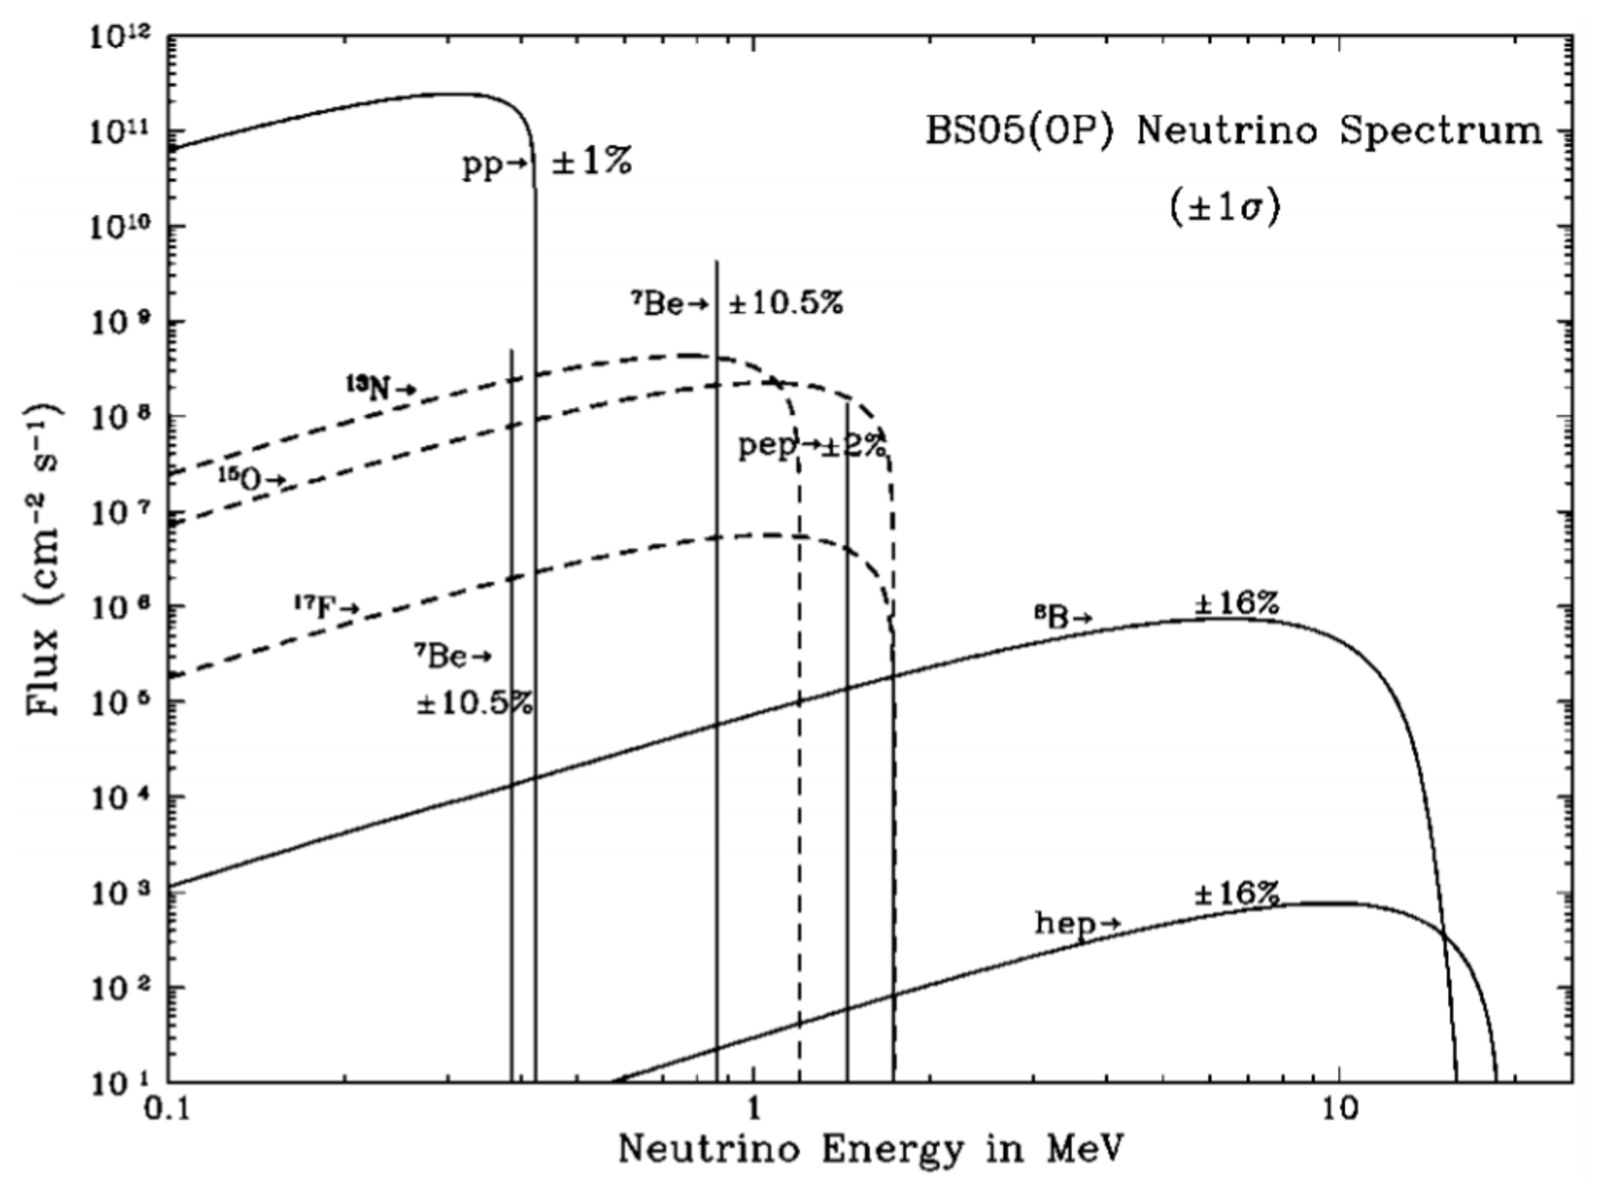
\includegraphics[width=10cm]{BP05.pdf}
	\caption{ Solar neutrino energy spectrum ($E_\nu$ vs. flux) for the solar model BS05(OP)\cite{BP05}.}
	\label{bp05plot}
\end{figure}

\subsection{Early Solar Neutrino Experiments}
In 1964, John Bahcall and Raymond Davis proposed the first experiment to detect solar neutrinos\cite{bahcall1,raymond}. Raymond Davis designed an experiment that used a 380 m$^3$ tank filled with Perchloroethylene (C$_2$Cl$_4$), a dry-cleaning fluid rich in chlorine. Solar neutrinos were expected to change $^{37}$C1 to $^{37}$Ar via the endothermic reaction $\nu_e+^{37}$Cl$\to^{37}$Ar$+e^-$ and the produced $^{37}$Ar were extracted and counted. The neutrino energy threshold ($E_{thresh}$) of the experiment was 0.814 MeV, which allowed a measurement mostly of the $^8$B neutrino flux but also including some lower energy neutrinos\cite{raymond}. Their first results, announced in 1968, showed that only about one-third of the predicted radioactive argon atoms were measured. This raised a problem of missing solar neutrinos.
\subsection{Atmospheric Neutrino}
Cosmic rays from outer space continuously interact with nuclei in the atmosphere and produce secondary particles. Atmospheric neutrinos come from decay products of the hadrons in the secondaries. The dominate processes of atmospheric $\nu_e$ and $\nu_\mu$ production is $\pi^+\to\mu^+ + \nu_\mu$ followed by $\mu^+ \to e^+ + \bar{\nu}_\mu + \nu_e$. In the 1980s, the Kamiokande experiment in Japan measured atmospheric neutrinos by utilizing a 3-kiloton water-Cherenkov detector. The incoming neutrinos, $\nu_e$ ($\nu_\mu$) interacted with the water via charged current interactions and electrons (muons) were produced. The electrically charged leptons traversed the water at a speed higher than the speed of light in water and thus emit Cherenkov light, which were recorded by the detector as ring patterns (called Cherenkov rings). The produced electrons caused electro-magnetic showers during their propagation in the water while the produced muons propagated almost in straight lines without producing electro-magnetic showers. Then the $\nu_\mu$ (the $\mu$-like events) were separated from the $\nu_e$ (the $e$-like events) by the fact that the $\mu$-like events created sharper Cherenkov rings than the $e$-like events. KamiokaNDE measured the ratio of fluxes $\Phi(\nu_\mu+\bar{\nu}_\mu)/\Phi(\nu_e+\bar{\nu}_e)$. The fluxes of atmospheric neutrinos are well understood and the ratio $\nu_\mu/\nu_e$ is expected to be $\sim$2 at low energies $\leq$1~GeV. In 1988, they found a deficit of measured $\mu$-like events compared to the prediction. This was later confirmed by IMB in 1992\cite{imb} and Soudan-2 in 1997\cite{soudan2} and called ``atmospheric neutrino anomaly''\cite{atmNuReview}.

\section{Neutrino Flavor Mixing and Conversion}
\subsection{SNO and Super-Kamiokande}
The deficit of solar neutrinos and atmospheric neutrinos indicate that a neutrino can change its flavor or oscillate during propagation.

To resolve the solar neutrino problem with a direct approach, Herbert Chen in 1984 proposed an experiment using a large heavy water (D$_2$O) Cherenkov detector to distinguish the flavors of solar neutrinos\cite{herbertChen}. This proposal lead to the SNO collaboration. The SNO detector was sensitive to the $^8$B solar neutrinos via three interactions: (1) the charged current (CC): $\nu_e+d\to e^-+p+p$ , (2) the neutral current (NC): $\nu_x+d\to\nu+p+n$, (3) the elastic scattering (ES): $\nu_x+e^-\to \nu_x+e^-$. The CC channel was only sensitive to $\nu_e$ while the NC channel was independent of the neutrino type, which provided a measurement of the total solar neutrino flux regardless of flavors. The ES channel was also sensitive to all flavors but with reduced sensitivities to $\nu_\mu$ and $\nu_\tau$\cite{SNO}.

In 2002, SNO reported that the measured total $^8$B solar neutrino flux via the NC channel ($\Phi_{NC}$) was consistent with solar models while the $\nu_e$ component of the flux ($\Phi_e$) was about one-third of the total flux\cite{SNO}. The results reported in 2013 was\cite{SNOresult}:
\[
P_{SNO} = \frac{\Phi_e}{\Phi_{NC}}= 0.340\pm0.023^{+0.029}_{-0.031}
\]

The results indicate that about two-thirds of the original solar $\nu_e$ have transformed to $\nu_{\mu,\tau}$ when they arrive at earth. This explains the problem of missing solar neutrinos.

In 1996, the Kamiokande experiment was upgraded to a 50-kiloton water Cherenkov detector, Super-Kamiokande (Super-K). In two years, Super-K measured atmospheric neutrinos and announced a striking discovery: the number of high energy muon neutrinos is zenith angle dependent and caused by a deficit of up-going $\nu_\mu$\cite{superK}. 

The measured up-going muon neutrinos are mostly created in the atmosphere at the opposite side of the Earth to the Super-K detector and travel about 12800 km while the downward-going muon neutrinos are created in the atmosphere about 15 km above the detector. The measured $\nu_e$ in the same scenario do not show such a deficit\cite{superK}.

Therefore, a natural explanation for the results is that the up-going muon neutrinos have oscillated to $\nu_\tau$ during their thousands of kilometres travel. The Super-K results are consistent with two-flavor $\nu_\mu\leftrightarrow\nu_\tau$ oscillations\cite{superK}.


\subsection{Flavor Mixing Matrix and Oscillation Probability}
Both SNO and Super-K discovered the phenomenon of neutrino flavor conversions directly and were awarded the 2015 Nobel Prize. The phenomenon proves that neutrinos have a small but finite mass. The violation of lepton number conservation is not expected in the Standard Model. As early as 1957, Pontecorvo had already suggested an oscillation of $\nu\leftrightarrow\bar{\nu}$, and later worked out a phenomenological model for $\nu_e\leftrightarrow\nu_\mu$ in theory\cite{nobeldoc}. In 1962, Ziro Maki, Masami Nakagawa and Shoichi Sakata further introduced a lepton mixing matrix (usually called the PMNS matrix), which is a unitary transformation relating the neutrino flavor and mass eigenstates, as a model for the mixing of different neutrino flavors\cite{oxfordneutrino}.

The flavor of a neutrino can be taken as a superposition of the mass eigenstates. The two-flavor neutrino mixing model in vacuum is a simplified way to discuss the phenomenon of neutrino flavor conversion.

For a mixing of flavor states $\nu_e$ and $\nu_\mu$, we have a $2\times2$ unitary matrix with a mixing angle $\theta$ to relate the flavor eigenstates to the mass eigenstates\cite{cahn}:
\begin{equation}\label{eq:2flavormatrix}
\begin{bmatrix}
\nu_e\\
\nu_\mu\\
\end{bmatrix}
= U\begin{bmatrix}
\nu_1\\
\nu_2\\
\end{bmatrix}, ~~U=\begin{bmatrix}
\cos\theta &\sin\theta\\
-\sin\theta &\cos\theta\\
\end{bmatrix}.
\end{equation}

The flavor states evolve in time according to $\nu_i(t) = e^{-iE_it}\nu_i(0)~(i = 1,2)$ (using natural unit, $\hbar=c=1$),
\begin{equation}
\begin{aligned}
|\nu_e(t)> = \cos\theta e^{-iE_1t}|\nu_1>+\sin\theta e^{-iE_2t}|\nu_2>
\\
|\nu_\mu(t)> = -\sin\theta e^{-iE_1t}|\nu_1>+\cos\theta e^{-iE_2t}|\nu_2>.
\end{aligned}
\end{equation}

Then the probability that a $\nu_e$ at time $t_0=0$ transforms to a $\nu_\mu$ at time $t$ is:
\begin{equation}
P_{\nu_e\to\nu_\mu} = |<\nu_\mu(t)|\nu_e(0)>|^2= 2\sin^2\theta\cos^2\theta[1-\cos(E_2-E_1)t].
\end{equation}

For ultra-relativistic neutrinos, the momentum $|\vec{p}|=p\simeq E\gg m$, then $E_1\simeq p+\frac{m^2_1}{2p}$ and $E_2\simeq p+\frac{m^2_2}{2p}$, we have $E_2-E_1\simeq\frac{m_2^2-m_1^2}{2p}$,
then $P_{\nu_e\to\nu_\mu}$ can be simplified to be:
\begin{equation}\label{eq:oscillation}
P_{\nu_e\to\nu_\mu} = \sin^2( 2\theta)\sin^2(\frac{m_2^2-m_1^2}{4E}t)=\sin^2( 2\theta)\sin^2(\frac{\Delta m^2}{4E}L),
\end{equation}
where $\Delta m^2=m_2^2-m_1^2$. $L = t$ is the distance neutrino travels. 

Maximum oscillation occurs at $\frac{\Delta m^2}{4E}L\sim \pi$, which gives an effective length $L^{osc}=4\pi E/\Delta m^2$.

For a set of units commonly used by experiments, a neutrino with energy $E_\nu$, after flying for a distance of $L$, has an oscillation probability of: 
\begin{equation}
P_{\nu_e\to\nu_{\mu}}=\sin^2(2\theta)\sin^2\Big(\frac{1.27\Delta m^2[eV^2]L[km]}{E_\nu[GeV]}\Big).
\end{equation}
The survival probability is defined as:
\begin{equation}
P_{\nu_e\to\nu_e}=1-P_{\nu_e\to\nu_{\mu}}.
\end{equation}

\subsection{Matter Effects}
The matter effect is caused by neutrinos interacting with ambient electrons and nucleons in matter such as the Sun or the Earth. $\nu_e$ interacts with electrons via both charged weak current (exchanging $W$ boson) and neutral weak current ($Z$ boson) while $\nu_\mu$ and $\nu_\tau$ interact only by the neutral current. The $\nu_e$ energy has an addition term, $V_{CC} =\sqrt2G_Fn_e$, where $n_e$ is the number density of the electrons in matter and $G_F$ is the Fermi coupling constant for the weak interaction. This effect affects the oscillation probabilities for neutrinos propagating in matter compared to vacuum, which is called the Mikheyev-Smirnov-Wolfenstein (MSW) mechanism\cite{smirnov,smirnov_msw}.

In vacuum two-flavor mixing, the Schr\"{o}dinger equation in flavor eigenstates can be written (in natural units)\cite{xing}:
\begin{equation}\label{eq:2flavor_simple}
i\frac{d}{dt}\begin{bmatrix}
\nu_e\\
\nu_\mu\\
\end{bmatrix}
=
H^f_0
\begin{bmatrix}
\nu_e\\
\nu_\mu\\
\end{bmatrix}
\end{equation}
where 
\begin{equation}\label{eq:H0f}
H^f_0 = \begin{bmatrix}
-\frac{\Delta m^2}{4E}\cos 2\theta & \frac{\Delta m^2}{4E}\sin 2\theta\\
\frac{\Delta m^2}{4E}\sin 2\theta &\frac{\Delta m^2}{4E}\cos 2\theta\\
\end{bmatrix}+\frac{(m_1^2+m_2^2)}{2}\begin{bmatrix}
1 & 0\\
0 &1\\
\end{bmatrix}
\end{equation}

To simplify the calculation, we can drop the second unitary term of $H^f_0$ that is irrelevant to the neutrino flavor conversion. Including the matter effect, we obtain:
\begin{equation}\label{eq:Hm}
H_m = \begin{bmatrix}
-\frac{\Delta m^2}{4E}\cos 2\theta+\sqrt 2G_Fn_e & \frac{\Delta m^2}{4E}\sin 2\theta\\
\frac{\Delta m^2}{4E}\sin 2\theta &\frac{\Delta m^2}{4E}\cos 2\theta\\
\end{bmatrix}
\end{equation}

We define a mixing angle in matter, $\theta_m$ as:
\begin{equation}\label{eq:thetaM}
\tan 2\theta_m = \frac{\Delta m^2\sin2\theta}{\Delta m^2\cos2\theta-2\sqrt 2E G_Fn_e},
\end{equation}
and define an effective squared-mass difference in matter $\Delta m^2_m$ as:
\begin{equation}
\Delta m^2_m = \sqrt{(\Delta m^2\cos2\theta - 2\sqrt 2EG_Fn_e)^2+(\Delta m^2\sin2\theta)^2}.
\end{equation}

In analogy with mixing in vacuum, we can write the mixing equation relating the energy eigenstates in matter ($\nu_{1m},\nu_{2m}$) to the flavor eigenstates with a diagonalized Hamiltonian:
\begin{equation}\label{eq:matter_mixing}
\begin{bmatrix}
\nu_e\\
\nu_\mu\\
\end{bmatrix}
= \begin{bmatrix}
\cos\theta_m & \sin\theta_m\\
-\sin\theta_m & \cos\theta_m \\
\end{bmatrix}
\begin{bmatrix}
\nu_{1m}\\
\nu_{2m}\\
\end{bmatrix}.
\end{equation}

The probability of flavor conversion in matter is:
\begin{equation}
P_{\nu_e\to\nu_{\mu}}=\sin^2(2\theta_m)\sin^2\Big(\frac{\Delta m_m^2L}{4E}\Big).
\end{equation}

The denominator in equation (\ref{eq:thetaM}) implies a resonance condition:
\begin{equation}\label{eq:reson_condition}
V(n_e)=\sqrt 2G_Fn_e=\frac{\Delta m^2\cos2\theta}{2E}.
\end{equation}

From this condition, for a given $E$, there is a resonance density $n^{reson}_e$ while for a given $n_e$, there is a resonance energy $E^{reson}$. When the resonance condition is satisfied, $\theta_m = \frac{\pi}{4}$ and two flavor neutrinos are maximally mixed, even if the vacuum mixing angle $\theta$ is small. This is called matter enhanced neutrino oscillation\cite{smirnov,japan_text}.

\subsection{Three-flavor mixing}
For three-flavor neutrino mixing, we have\cite{pdg2018}:
\begin{equation}\label{eq:mixingmatrix}
|\nu_f> = \sum_{k=1}^3U^*_{fk}|\nu_k>, 
\end{equation}
where $f=e,\mu,\tau$ and $k=1,2,3$. The unitary PMNS matrix, $U_{PMNS}$, can be parametrized as: 
$U_{PMNS} = $
\begin{equation}
\begin{bmatrix}
1 &0 &0\\
0 &\cos\theta_{23} &\sin\theta_{23}\\
0 &-\sin\theta_{23} &\cos\theta_{23}\\ 
\end{bmatrix}
\begin{bmatrix}
\cos\theta_{13} &0 &e^{-i\delta_{CP}}\sin\theta_{13}\\
0 &1 &0\\
e^{-i\delta_{CP}}\sin\theta_{13} &0 &\cos\theta_{13}\\ 
\end{bmatrix}
\begin{bmatrix}
\cos\theta_{12} &\sin\theta_{12} &0\\
-\sin\theta_{12} &\cos\theta_{12} &0\\
0 &0 &1\\ 
\end{bmatrix}.
\end{equation}

In the PMNS matrix, we have four parameters: the three mixing angles $\theta_{12}$, $\theta_{13}$, $\theta_{23}$ and the charge-parity (CP) violation parameter of lepton sector, $\delta_{CP}$. The unknown value of $\delta_{CP}$ is related to leptogenesis, the hypothetical physical process that produced an asymmetry between leptons and antileptons in the very early universe\cite{wiki_cp}. In addition, there are two squared-mass differences, $\Delta m^2_{21}=m_2^2-m_1^2$ and $\Delta m^2_{32}=|m_3^2-m_2^2|$. The sign of $\Delta m^2_{32}$ is unknown and it indicates a mass hierarchy problem of whether neutrino mass is normal hierarchy (NH, $m_3>m_2>m_1$) or inverted hierarchy (IH, $m_3<m_1<m_2$)\cite{pdg2018}. 

Currently, these six parameters have been measured by neutrino oscillation experiments. These experiments can be classified by the neutrino sources they use. They are the solar, the reactor, the atmospheric, the accelerator and the astronomical neutrino experiments. Table~\ref{nu_exp} lists the energy scale of the neutrino source as well as the example experiments.

\begin{table}[ht]
	\caption{\label{nu_exp} Oscillation neutrino experiments.}	
	{\centering
		\begin{tabular*}{135mm}{c@{\extracolsep{\fill}}cccc}
			\toprule 
		type & source & $E_\nu$ & example\\
			\midrule
		solar& the Sun & MeV scale & SNO \\
		reactor& reactor & MeV scale & DayaBay \\
		atmospheric& cosmic-ray& GeV scale & SuperK\\
		accelerator&  $\nu$ beam from accelerator & GeV scale & T2K\\	
		astronomical& astronomical objects & GeV-EeV scale & IceCube\\	
			\bottomrule	
		\end{tabular*}
	}
\end{table}

For the $\Delta m^2_{21}$ and $\theta_{12}$, the combined analysis of the measurements from the reactor experiment KamLAND and SNO gave $\Delta m^2_{21} = 7.59^{+0.21}_{-0.21}\times 10^{-5}eV^2$ and $\tan^2{\theta}_{21}=0.47^{+0.06}_{-0.05}$\cite{kamland_measure}.

The accelerator neutrino experiments as well as the atmospheric neutrino experiments have measured $\Delta m^2_{32}$ and $\theta_{23}$. The most recent results from SuperK show that in NH, $\sin^2\theta_{23}=0.588^{+0.031}_{-0.064}$ and $\Delta m^2_{32} = 2.5^{+0.13}_{-0.20}\times 10^{-3} eV^2$\cite{superk_new}. 

In 2012, the reactor neutrino experiment Daya Bay reported the discovery of non-zero $\theta_{13}$ with a significance of 5.2$\sigma$. In 2016, Daya Bay reported that $\sin^2 2\theta_{13} = 0.0841\pm0.0027(stat.)\pm0.0019(syst.)$. This high-precision result makes $\sin^2 2\theta_{13}$ the best measured mixing angle\cite{dayabayresults,reactorNu}.

$\delta_{CP}$ is examined by the experiments which measure the difference between neutrino and antineutrino oscillation probabilities $P(\bar{\nu}_\alpha\to\bar{\nu}_\beta)$ and $P(\nu_\alpha\to\nu_\beta)$\cite{xing}. In 2017, the T2K experiment in Japan rejected the hypothesis that neutrinos and antineutrinos oscillate with the same probability at 95\% confidence (2$\sigma$) level. This indicates a hint of CP symmetry broken by neutrinos\cite{t2k}.

\section{Double Beta Decay}

For heavy radioactive isotopes with nuclei of even neutron number (N) and even proton number (Z) (called even-even nucleus), beta decay will lead to an odd-odd nucleus which is less stable. For some such isotopes the beta decay is energetically forbidden. In 1935, Maria Goeppert-Mayer pointed out that they can still decay through a double beta decay process: $(Z,A) \to (Z+2,A)+2e^{-}+2\bar{\nu_e}$. This is called ordinary double beta decay or $2\nu\beta\beta$\cite{martin}.

In 1937, Ettore Majorana proposed that neutral spin-1/2 particles (fermions) can be their own antiparticles\cite{majorana}. If neutrinos have this behaviour, the process called neutrinoless double beta decay ($0\nu\beta\beta$) will also be expected. The Feynman diagrams of $2\nu\beta\beta$ and $0\nu\beta\beta$ are illustrated in Figure~\ref{feynman1}.

\begin{figure}[htbp]
	\centering	
	\begin{minipage}[t]{0.45\textwidth}
	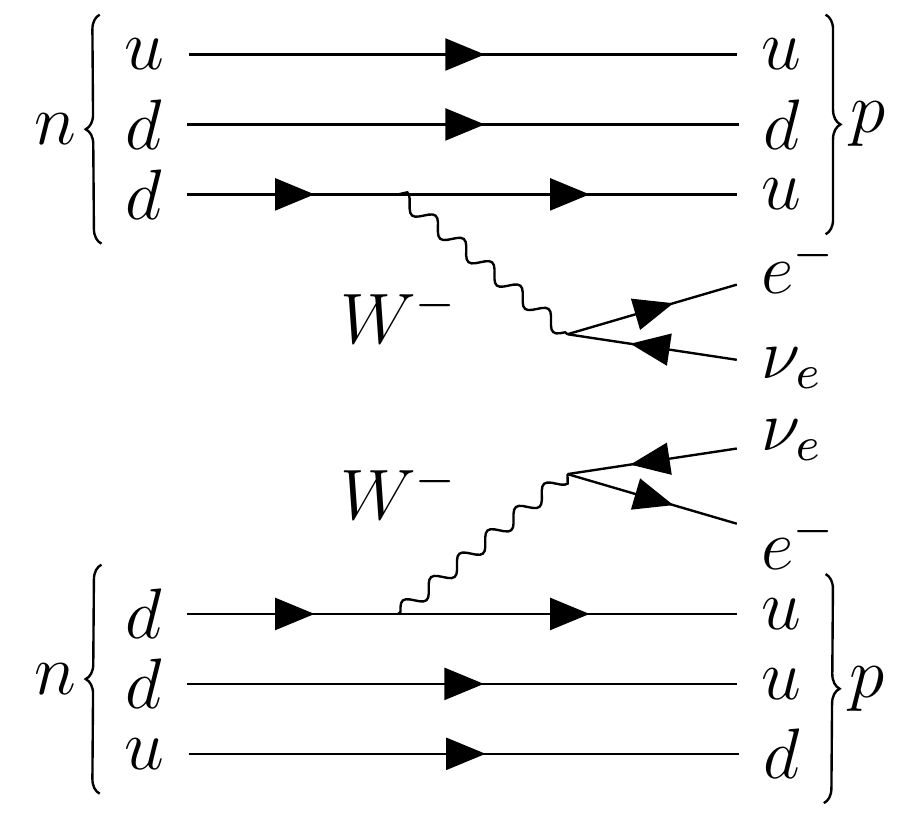
\includegraphics[width=5cm]{doubleBeta2nu_feynman.png}
	\end{minipage}
	\begin{minipage}[t]{0.45\textwidth}
	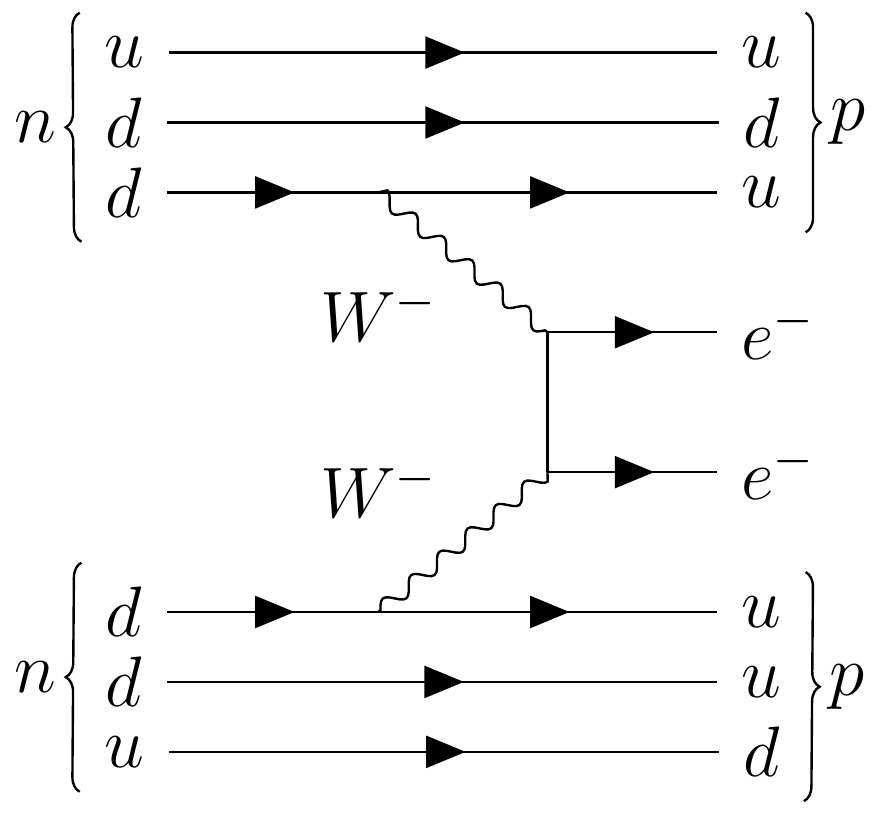
\includegraphics[width=5cm]{doubleBeta_feynman.png}
	\end{minipage}
	\caption{ Feynman diagrams for $2\nu\beta\beta$ (left) and $0\nu\beta\beta$ (right).}
	\label{feynman1}
\end{figure}

The interpretation of the $0\nu\beta\beta$ process is considered as exchanging light Majorana neutrinos. In this case the effective Majorana mass $<m_{ee}>=\sum_{i=1}^{3} |U_{ei}|^2m_i~(i=1,2,3)$, $U_{ei}$ are the elements of the neutrino mixing matrix for the flavor state $\nu_e$, and $m_i$ are the mass eigenvalues of the mass eigenstates (from (\ref{eq:mixingmatrix})). The observable quantity is the half-life:
\[
(T^{0\nu\beta\beta}_{1/2})^{-1} = G_{PS}|M_{Nuclear}|^2<m_{ee}>^2, 
\]
where $G_{PS}$ is the phase space factor and $|M_{Nuclear}|$ is the nuclear matrix element for the physics process describing the $0\nu\beta\beta$ decay process\cite{kaizuber}.

Similar to beta decay, the $2\nu\beta\beta$ process will cause a continuous spectrum in the detector while the $0\nu\beta\beta$ process only has two electrons in the final state, which sum up to give a distinct energy peak. By measuring this exact energy, a detector with high energy resolution is able to search for the $0\nu\beta\beta$ signal from the $0\nu\beta\beta$ decay radioactive isotopes. Diverse technologies have been developed during the past decades. The following section lists some of the mainstream experiments.

\subsection{Status of Double Beta Decay Experiments}
The GERmanium Detector Array (GERDA) experiment searches for $0\nu\beta\beta$ of $^{76}$Ge. The experiment uses bare germanium crystals with an enrichment of up to $\sim$87\% $^{76}$Ge operated in radiopure cryogenic liquid argon (LAr). In 2017, GERDA reported a 90\% confidence level (C.L.) lower limit for the half-life of $^{76}$Ge, $T^{0\nu}_{1/2}(^{76}$Ge$)>8.0\times 10^{25}$ years\cite{gerda,gerda2,gerda2018}.

The Enriched Xenon Observatory (EXO) experiment uses 200-kg of liquid Xenon (LXe) in a time projection chamber (TPC) to search for $0\nu\beta\beta$ in $^{136}$Xe. In 2011 they observed the half life of $2\nu\beta\beta$ of $^{136}$Xe to be $2.11\times 10^{21}$ years. A limit of $T^{0\nu}_{1/2}(^{136}$Xe$)>1.1\times 10^{25}$ yr\cite{exo} was set in 2014. EXO is now being upgraded to the next 5-ton experiment (nEXO) and is expected to reach an exclusion sensitivity of $T^{0\nu}_{1/2}(^{136}$Xe) of about $10^{28}$ years at 90\% C.L.\cite{nEXO}.

Also using $^{136}$Xe, the KamLAND-Zen experiment exploits the existing facilities of KamLAND by setting a 3.08-m-diameter spherical inner balloon filled with 13 tons of Xe-loaded liquid scintillator at the center of the KamLAND detector. Their 2016 results from a 504 kg$\cdot$yr exposure obtained a lower limit for the $0\nu\beta\beta$ decay half-life of $T^{0\nu}_{1/2}(^{136}$Xe$)>1.07\times 10^{26}$ yr at 90\% C.L. and the corresponding upper limits on the effective Majorana neutrino mass are in the range 61-165 meV\cite{kamlandZen}.

The Cryogenic Underground Observatory for Rare Events (CUORE) experiment searches for $0\nu\beta\beta$ in $^{130}$Te. CUORE is a tonne-scale cryogenic bolometer array that arranges 988 tellurium dioxide (TeO$_2$) crystals. CUORE reported first results in 2017 after a total TeO$_2$ exposure of 86.3 kg$\cdot$yr. Combined with their early data, they placed a lower limit of $T^{0\nu}_{1/2}(^{130}$Te$)>1.5\times 10^{25}$ yr at 90\% C.L. and $m_{\beta\beta}<(140-400)$  meV\cite{cuore}.

The limits of $T^{0\nu}_{1/2}$ and $m_{\beta\beta}$ at 90\% C.L. from the above mentioned experiments are summarized in Table~\ref{gerdatable}\cite{gerda2018}.
\begin{table}[ht]
	\caption{\label{gerdatable} The limits of $T^{0\nu}_{1/2}$ and $m_{\beta\beta}$ at 90\% C.L.}	
	{\centering
		\begin{tabular*}{135mm}{c@{\extracolsep{\fill}}cccc}
			\toprule 
			Experiment & Isotope & Limit of $T^{0\nu}_{1/2}$ ($10^{25}$ year) & Limit of $m_{\beta\beta}$ (eV)\\
			\midrule
			GERDA       & $^{76}$Ge & $>$8.0 & $<$0.12-0.26  \\	
			KamLAND-Zen & $^{136}$Xe & $>$10.7 & $<$0.05-0.16	\\
			EXO         & $^{136}$Xe & $>$1.1 & $<$0.17-0.49  \\	
			CUORE       & $^{130}$Te & $>$1.5 &  $<$0.11-0.50 \\	
			\bottomrule	
		\end{tabular*}
	}
\end{table}
\vspace{1cm}
\section{SNO+ Experiment}
The SNO+ experiment is the successor of the SNO experiment, which makes use of the SNO detector structure. Located in SNOLAB at a depth of 2 km from the surface, the rock overburden is about 6000 meter water equivalent (m.w.e), which greatly reduces the cosmic muon backgrounds. The detector consists of an acrylic vessel (AV) sphere of 12 m in diameter and 5.5 cm in thickness. The AV sphere is concentric within a 17.8 m diameter stainless steel sphere, which holds 9438 photomultipliers (PMT). These two structures are housed in a rock cavity filled with 7000 tonnes of ultra-pure water (UPW) to provide both buoyancy for the vessel and radiation shielding\cite{whitepaper, erica}.

The SNO+ detector is designed for multi-purpose measurements of the neutrino physics.
The experiment will go through three phases\cite{whitepaper}: 

1. Water phase 

The AV was filled with about 900 tonnes of ultra-pure water. The detector has been collecting physics data since May 2017.

The main physics goal in this phase is to search for the invisible nucleon decay, which violates baryon number and is a prediction of Grand Unified Theory (GUT). In this decay mode, $^{16}$O decays into $^{15}$O$^*$ or $ ^{15}$O$^*$, which de-excites and produces a $\gamma$ ray of about 6 MeV.

During the water phase, different types of calibration runs have been taken. The detector responses, systematics and backgrounds are studied. Multiple physics analyses of solar neutrinos, reactor antineutrinos and nucleon decay are going on. The external backgrounds are also measured, which will be the same. 

2. Scintillator phase

The AV will be filled with 780 tonnes of liquid scintillator, which is a mixture of linear alkylbenzene (LAB) as a solvent and 2 g/L of 2,5-diphenyloxazole (PPO) as a fluor.

In this phase, the main physics goal is to measure low energy solar neutrinos: the CNO, pep and low energy $^8$B neutrinos. The pep neutrinos are mono-energetic, with $E_\nu$=1.442 MeV and their flux is well predicted by the Standard Solar Model. A measurement of the pep neutrinos will give more information of the matter effects in neutrino oscillations\cite{borexino}. 

The solar metallicity is the abundance of elements heavier than $^4$He (called ``metal'' elements in the context of astronomy). It is poorly constrained and the predictions from different solar models disagree with each other. A measurement of the CNO neutrinos can give the abundance of $^{12}$C, $^{13}$N and $^{15}$O and thus can resolve this problem\cite{cno}.

Geoneutrino, reactor antineutrino and supernova neutrino detections are additional goals.

A six-month period of scintillator filling and six to twelve months of data-taking is expected for this phase. During the filling, it is planned to operate the partially filled detector at a water level about 4.4 m for about two weeks. This partial filled transition phase is mainly aimed to understand the in-situ backgrounds of scintillator. 

3. Tellurium loading phase

In this final phase, natural Tellurium will be loaded into the scintillator, in which $^{130}$Te is a double beta decay isotope. The main purpose in this phase is searching for $0\nu\beta\beta$ in $^{130}$Te.

\section{My Work on SNO+}
\subsection{Wavelength Shifter (WLS) Study}
There was a proposal of adding wavelength shifter (WLS) into the SNO+ detector during the water phase. The specific wavelength shifter we considered is PPO, which will also be used in the SNO+ scintillator phase and Te-loaded phase. Although the proposal will not happen for SNO+ due to the experiment schedule, it is still worthwhile for a conceptual study of a SNO+-like detector that uses water-based wavelength shifter (wbWLS) as medium. The advantage of a wbWLS detector is to increase the light yield while still keeping the directionality. This technology is being studied by some future solar neutrino experiments, such as the Advanced Scintillation Detector Concept (ASDC)\cite{Dai,asdc}.

Figure~\ref{pmt_wls} shows the PMT distributions of Monte Carlo (MC) simulated 5 MeV electrons travelling along one direction (positive x axis) in the AV. The left plot shows the case when the detector is filled with pure water while the right plot is for water plus 0.1 ppm PPO. For the same electrons, the number of triggered PMTs (NHit) in waterPPO is about 2.4 times that in pure water. Although there is extra isotropic light emitted, the Cherenkov ring still can be seen clearly, allowing reconstruction of the directionality.  

\begin{figure}[htbp]
	\centering
	\begin{minipage}[t]{0.48\textwidth}
		\centering
		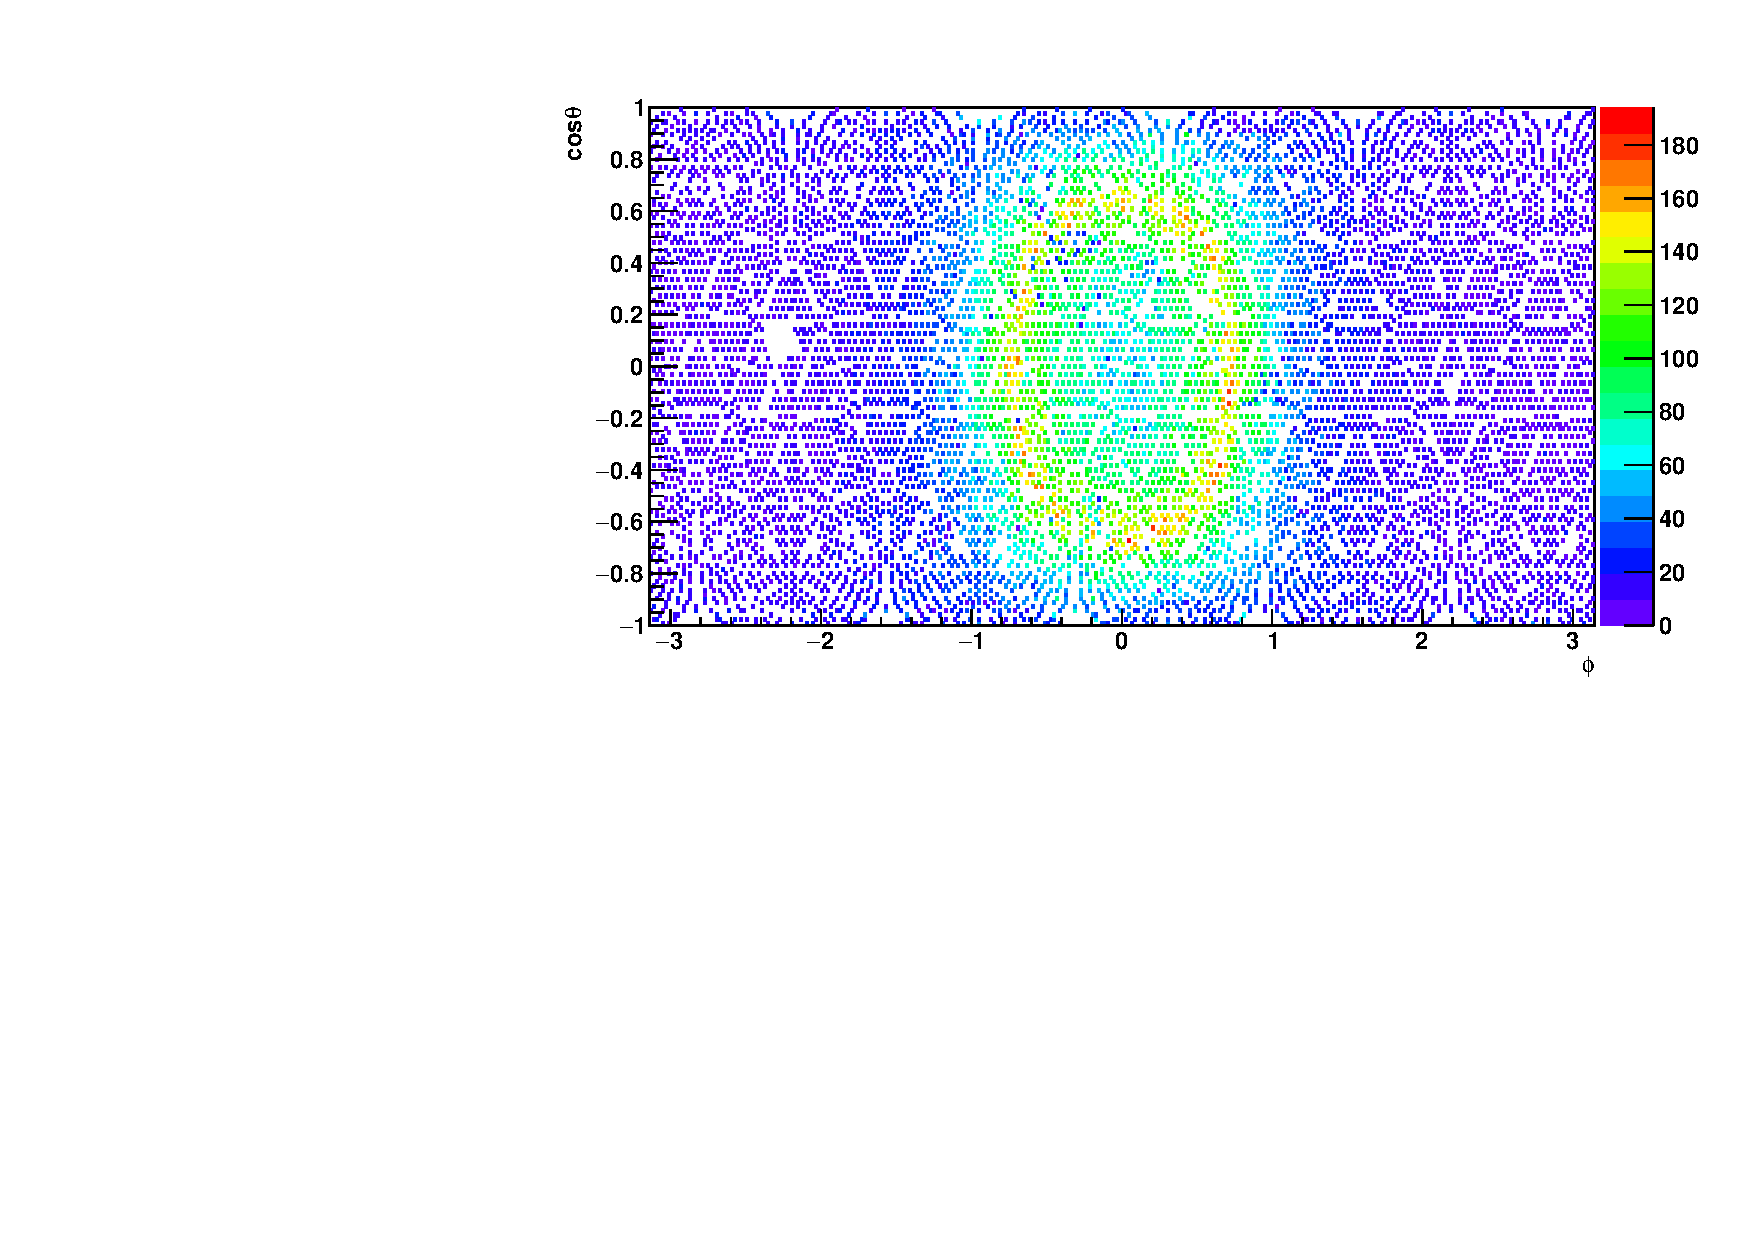
\includegraphics[width=7cm]{PMT_5MeVElectronWater.pdf}
	\end{minipage}
	\begin{minipage}[t]{0.48\textwidth}
		\centering
		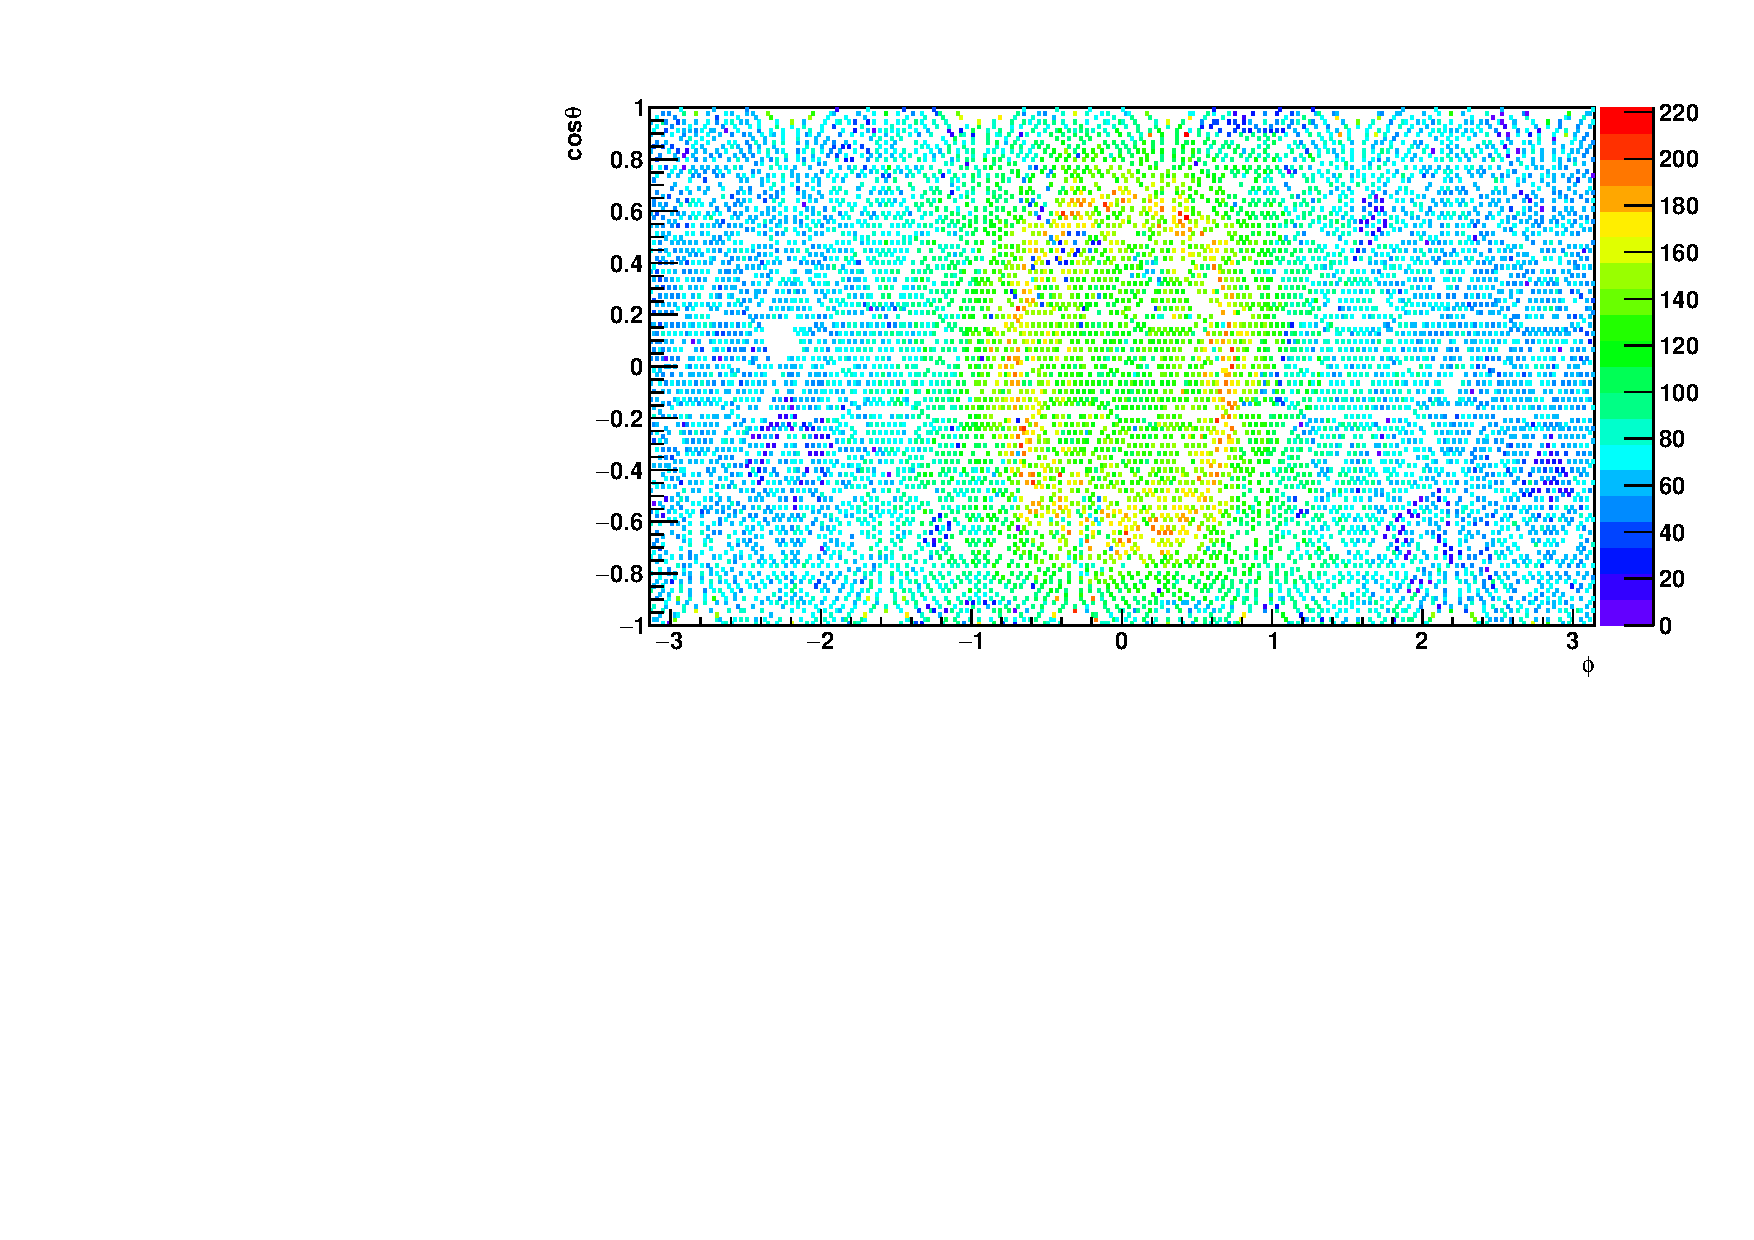
\includegraphics[width=7cm]{PMT_5MeVElectron0p1ppmPPO.pdf}
	\end{minipage}
	\caption{Distributions of PMT hit for 5 MeV electrons travelling along +x direction in the pure water (left); water plus 0.1 ppm PPO (right).}
	\label{pmt_wls}
\end{figure}

Figure~\ref{nhit_wls} shows the energies of simulated electrons as a function of the mean value of the Nhits distribution (mean Nhits). In pure water, a 1 MeV electron simulation does not trigger any PMTs while in wbWLS case we have a mean Nhits of 20.

\begin{figure}[htbp]
	\centering	
	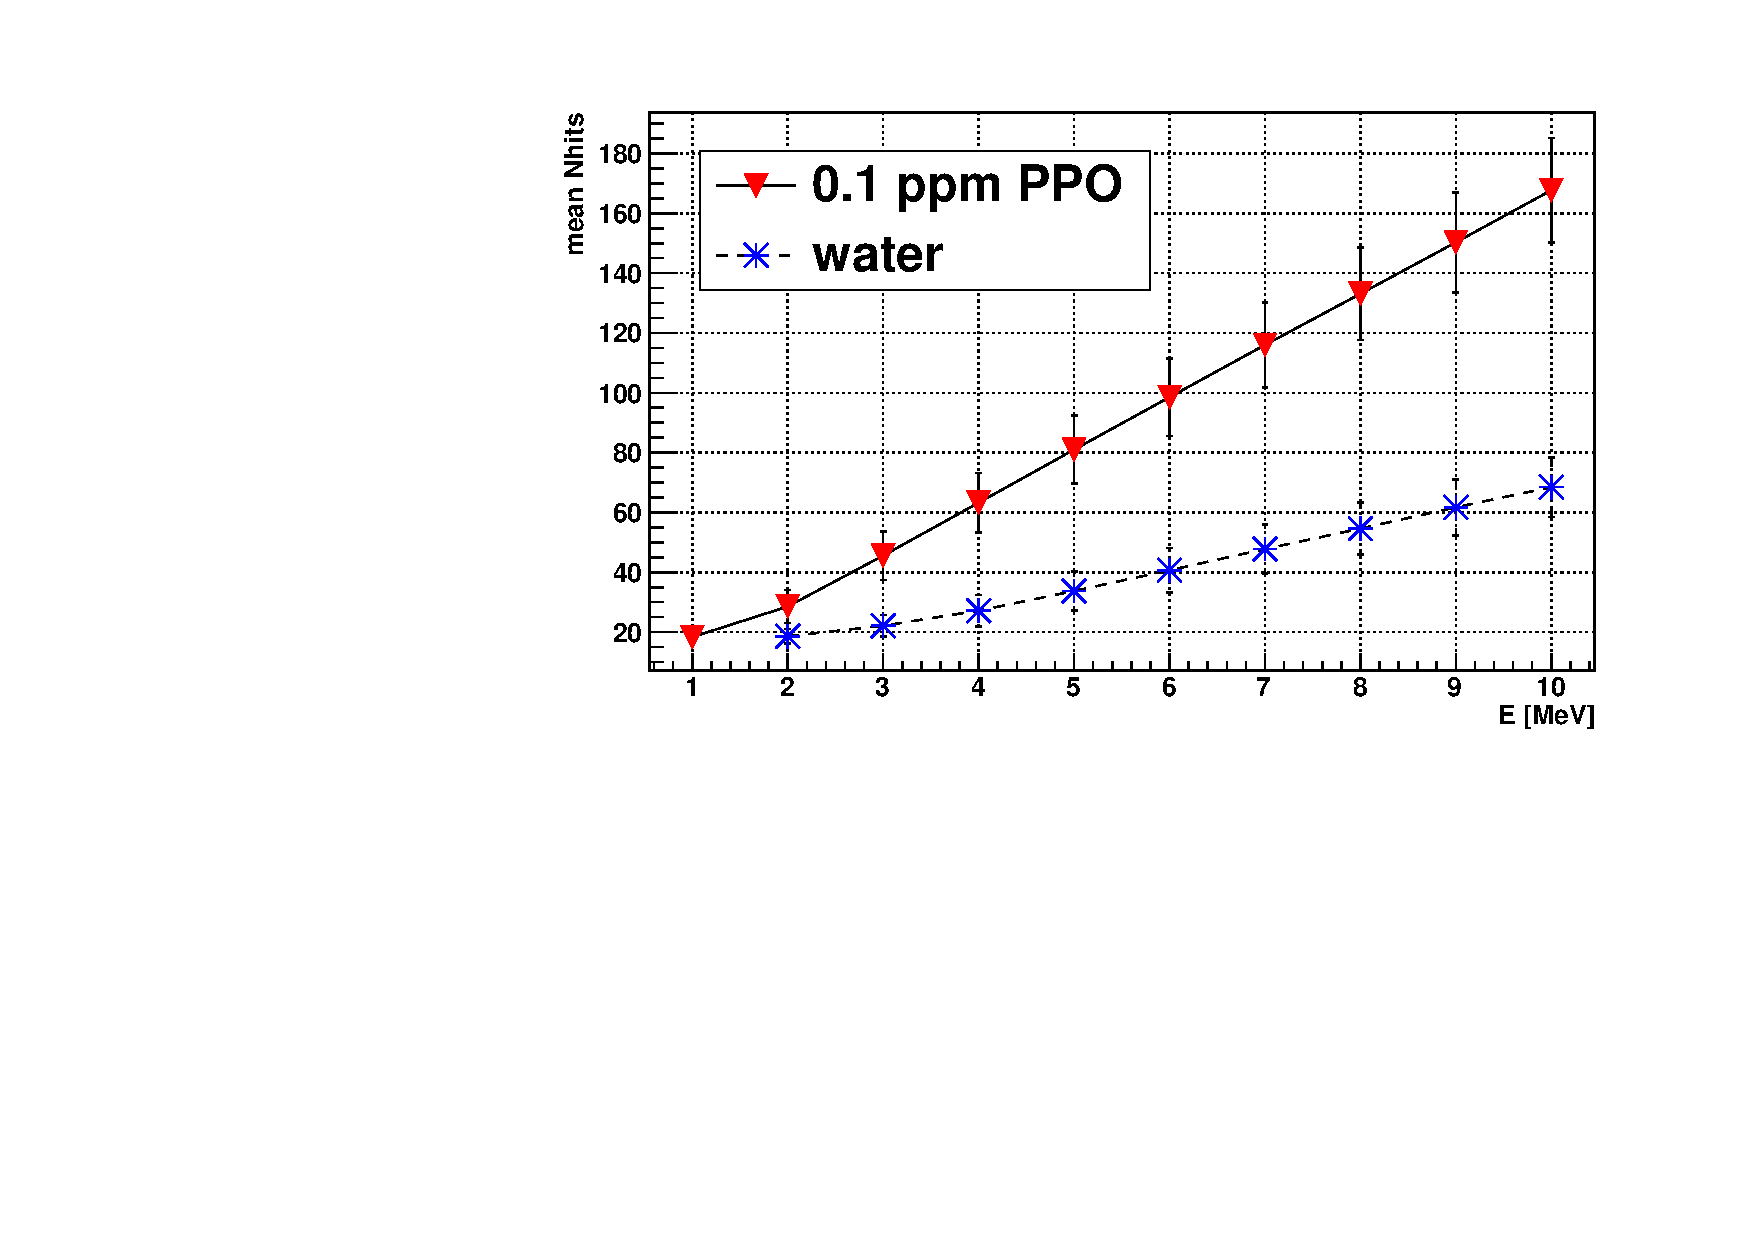
\includegraphics[width=9cm]{nhits_wls.pdf}
	\caption{ The energies of simulated electrons as a function of mean Nhits. The values in the 0.1 ppm PPO (solid line with inverted triangle) are compared with the water (dashed line with star).}
	\label{nhit_wls}
\end{figure}

To study the physics events in the wbWLS SNO+ detector, a reconstruction algorithm (fitter) is needed to obtain the position, direction and time of an event. A Multi-path Fitter (MPF) framework was developed by the Alberta group as an alternative fitter to the official one for SNO+. The fitter uses prompt light and straight line paths for likelihood calculations. Figure~\ref{mpwdiagram} shows the reconstruction concepts for position and direction. 

\begin{figure}[htbp]
	\centering
	\begin{minipage}[t]{0.45\textwidth}
		\centering
		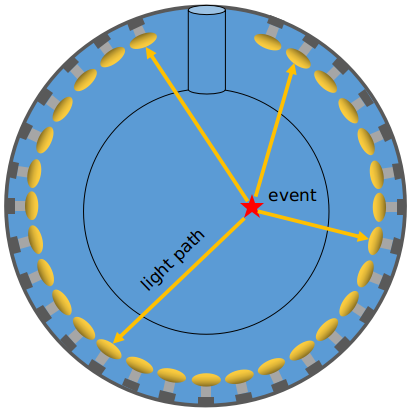
\includegraphics[width=5cm]{mpwDiagram.png}
	\end{minipage}
	\begin{minipage}[t]{0.4\textwidth}
		\centering
		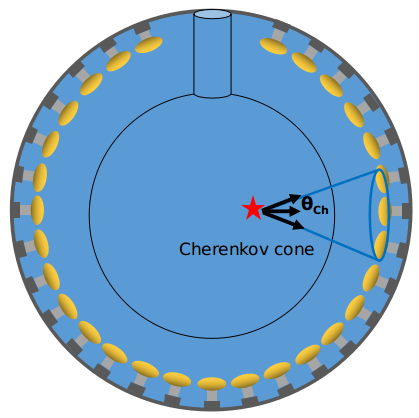
\includegraphics[width=5cm]{mpwDiagram2.png}
	\end{minipage}
	\caption{Diagrams of position reconstruction (left) and direction (right).}
	\label{mpwdiagram}
\end{figure}

In the left panel of Figure~\ref{mpwdiagram}, when an event happens at a position of $\vec{X}_{0}$, photons are emitted and propagate to PMTs. The triggered PMTs at known positions $\vec{X}_\mathrm{PMT}$ record the time when they fired ($t_\mathrm{PMT}$). The time residual is defined by: 
\begin{equation}
t_{res} = t_\mathrm{PMT}-\frac{|\vec{X}_{0}-\vec{X}_\mathrm{PMT}|}{v_{gr}}-t_0,
\end{equation}
where $t_0$ is the event time and $v_{gr}$ is an averaged group velocity of light.

For all the triggered PMTs, the likelihood is built by $L=\prod^{Nhit}_{i=0}P_i(t_{res})$, where $P_i$ is the calculated probability for the $i$-th triggered PMT based on $t_{res}$. If we know the timing spectrum of PMT response to a certain detector optical property, we can use the timing spectrum as a probability density function (pdf). For wbWLS the pdf is the PMT timing response modified by the photon propagation in the wbWLS. This timing pdf is shown in the left panel of Figure~\ref{WLS_pdf}.
The fitter varies the trial vertex of event position $\vec{X}_{0}$ and event time $t_0$, $(\vec{X}_{0},t_0)$ to calculate the likelihood function. By maximizing the likelihood, the best-fit vertex is found.

A cone of Cherenkov photons is created along the charged particle momentum $\vec{p}$, or the direction of the particle, $\hat n = \vec p/|\vec p|$. The light cone is detected on the PMT sphere, forming a Cherenkov ring. For a known (or best-fit) $\vec{X}_{0}$ and triggered PMT position $\vec{X}_{PMT}$, the angle $\theta_\mathrm{cone}$ between $(\vec{X}_{PMT}-\vec{X}_{0})$ and $\hat n$ is calculated by:
\[\cos\theta_\mathrm{cone} = \frac{(\vec{X}_\mathrm{PMT}-\vec{X}_{0})\cdot \hat{n}}{|\vec{X}_\mathrm{PMT}-\vec{X}_{0}|}.\]

It should be close to the Cherenkov angle $\theta_{Ch}$. This is illustrated in the right panel of Figure~\ref{mpwdiagram}. From MC simulations of electrons travelling along the same direction (positive x axis) in the pure water, we extract a distribution of $\cos\theta_{Ch}$ (angular distribution), as shown in the right panel of Figure~\ref{WLS_pdf}. It is peaked at $\cos\theta_{Ch}\approx 0.75$ ($\theta_{Ch}\approx 41.4^\circ$), which is the same as the water Cherenkov angle $\cos\theta_{Ch}=1/1.33$.

\begin{figure}[htbp]	
	\centering		
		\begin{minipage}[b]{0.5\textwidth}			
			%\centering			
			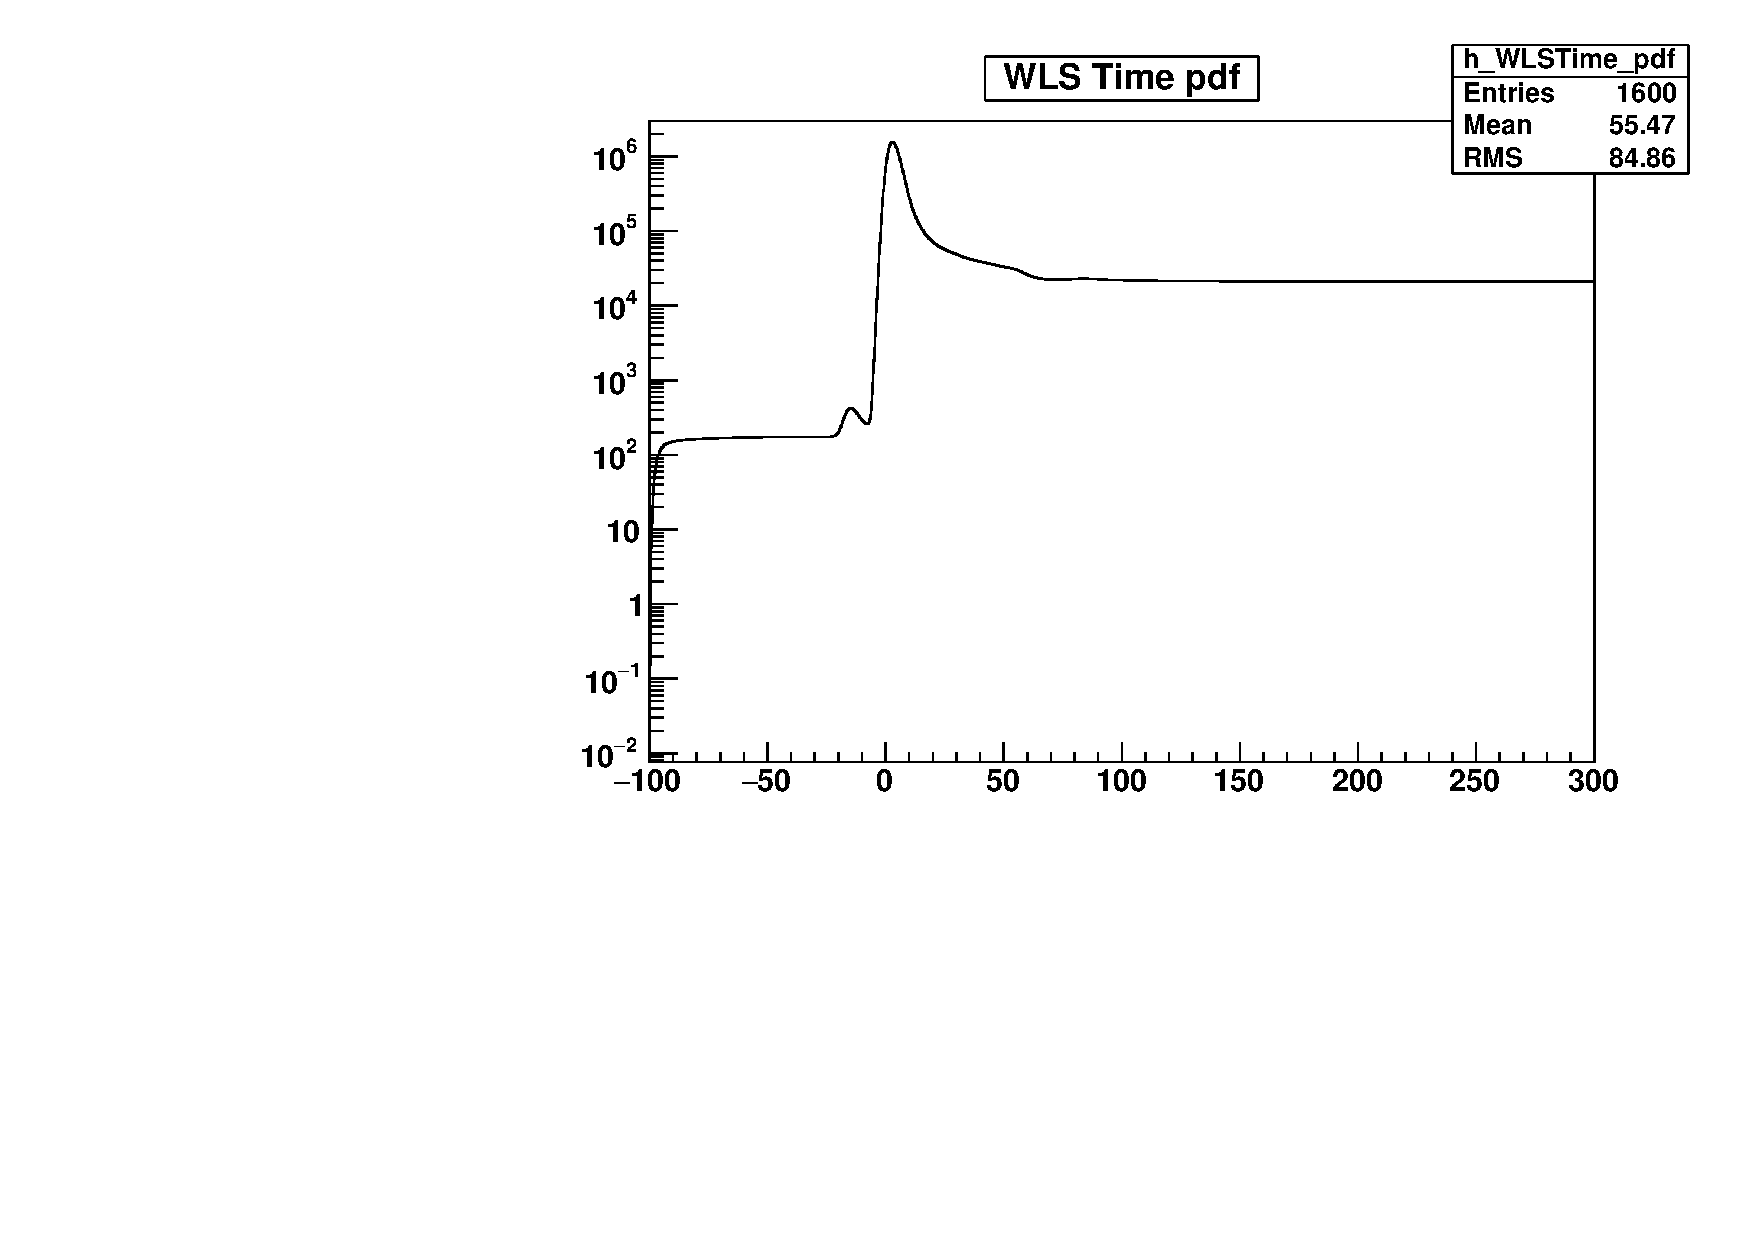
\includegraphics[height=5cm]{WLSTime_pdf.pdf}			
		\end{minipage}%				
		\begin{minipage}[b]{0.5\textwidth}		
			%\centering	
			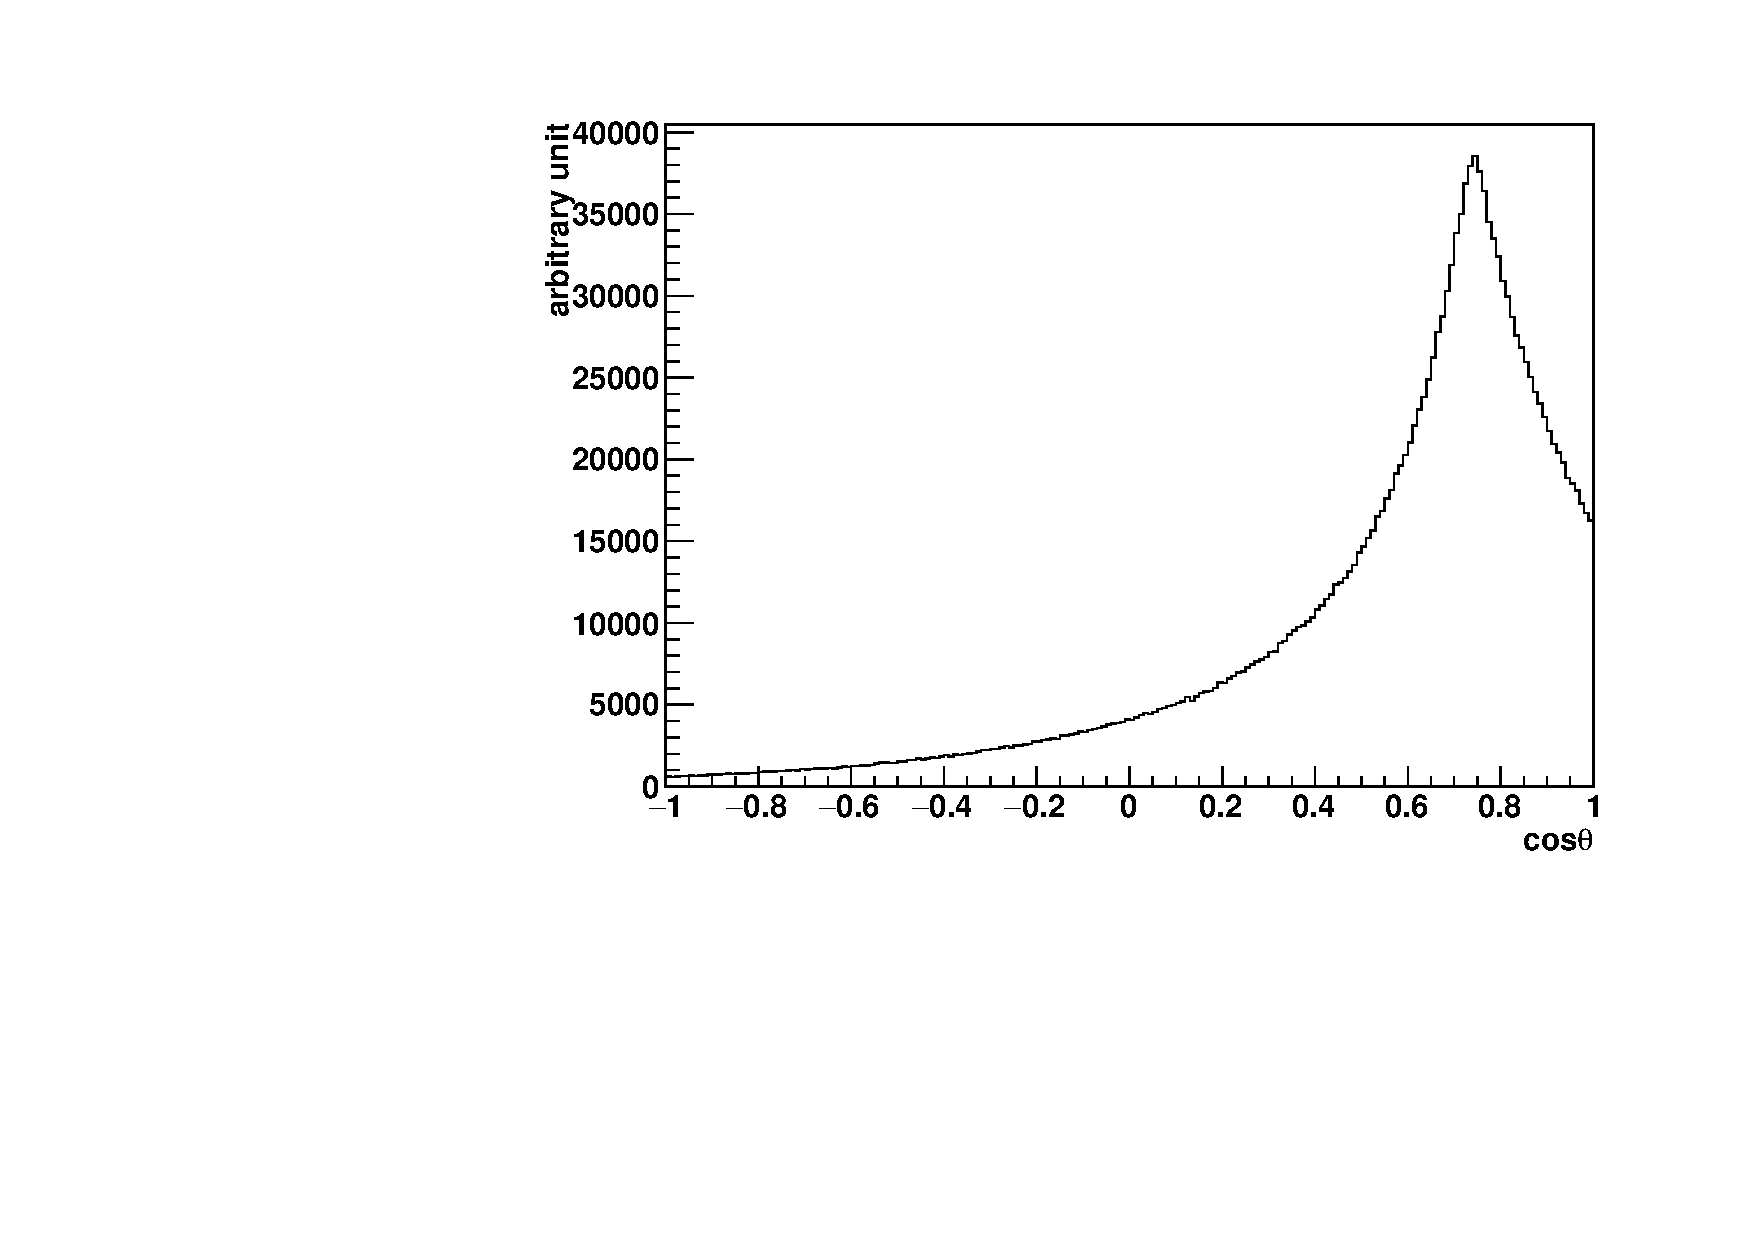
\includegraphics[height=5cm]{ChAngle_pdf.pdf}	
		\end{minipage}	
	\caption{\label{WLS_pdf} The distributions of the pdfs for wbWLS reconstruction. Left: the pdf of the WLS timing spectrum. Right: angular distribution caused by Cherenkov effect in pure water.}	
\end{figure}

In the wbWLS case, since WLS absorbs and re-emits photons, the above situations are slightly modified to build a WLS fitter. According to the optical property of PPO, the prompt light emitted from an event has a probability of $\sim$0.6 to be absorbed by the WLS and then re-emitted at a shifted vertex along the particle direction $\hat{n}$. Then the fitter returns a shifted vertex, $\vec{X}_{0,shifted}=\vec{X}_0+\mathrm{offset}\cdot\hat{n}$.  
The offset we set in the fitter is 100 mm obtained from simulation. 

To reconstruct the direction, we also need to consider the fraction of the re-emitted and wavelength shifted isotropic light.

To test the WLS fitter performance, 5 MeV electrons were simulated at the center of the AV filled with wbWLS and travelling along +x direction. As a comparison, the same simulation was done for the AV filled with pure water. For the pure water case, the events were reconstructed by the SNO+ official water fitter.

Figure~\ref{WLSFitPos} shows the performance of the WLS fitter reconstructed positions of the MC simulations compared to the pure water case. For the fit position distribution of 5 MeV electrons in the wbWLS, we get a root mean square (RMS) of 201 mm and a bias to the center (the mean of histogram) of 29 mm. Compared to the pure water case, the fit bias is about 19 mm better and the RMS is 188 mm better.

\begin{figure}[htbp]	
	\centering			
	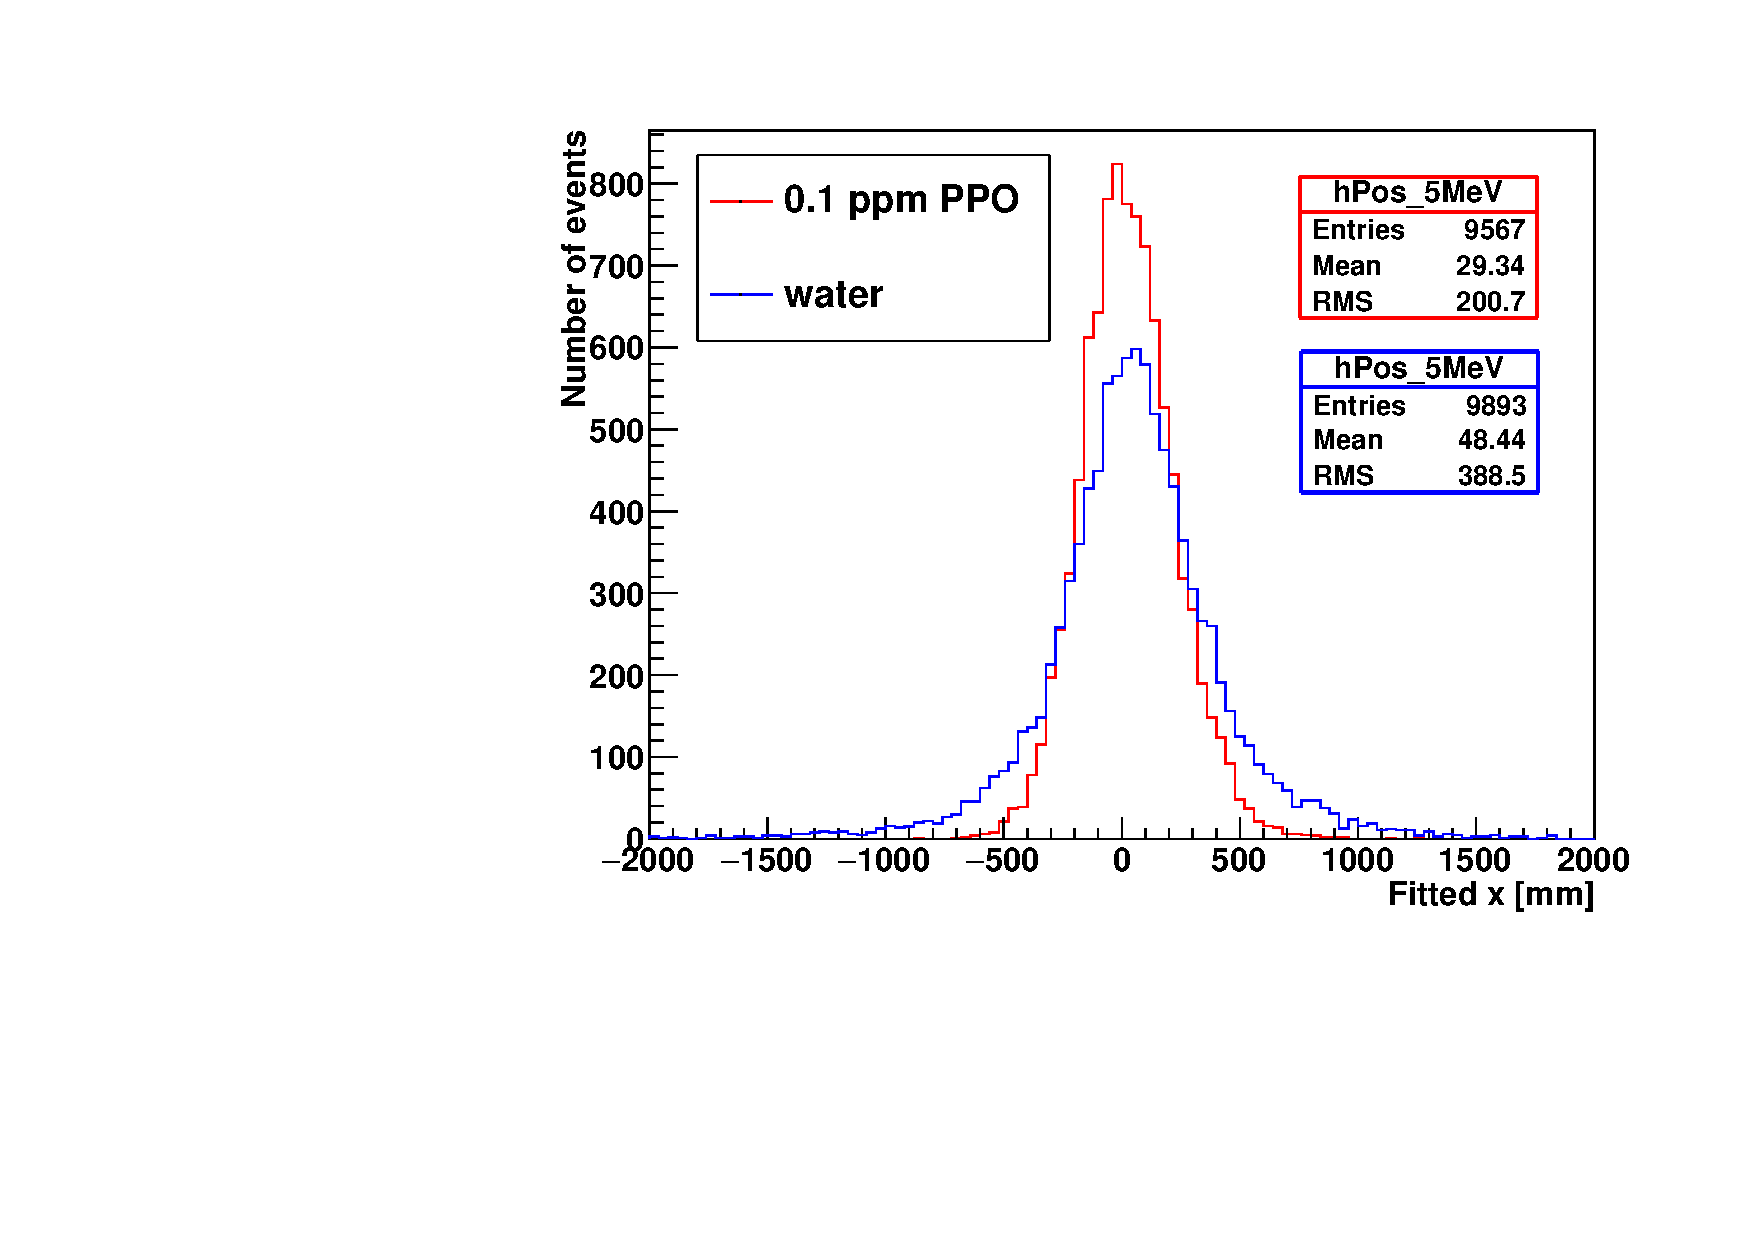
\includegraphics[height=5cm]{WLS_FittedPos.pdf}		
	\caption{\label{WLSFitPos} Fit position projected on x axis. The WLS fitter reconstructed X positions of the 5 MeV electron events in the wbWLS (red) are compared to the ones in the water (blue).
	}
\end{figure}

For a given Cherenkov event, the error in the reconstructed event direction is defined as\cite{boulay}: $\cos(\theta_e)=\vec{u}_{fit}\cdot\vec{u}_e$, where $\vec{u}_e$ is the simulated electron direction and $\vec{u}_{fit}$ is the reconstructed direction. To quantify this error, we define a $\cos\theta_{a}$ so that:
\[
\frac{\int_{\cos\theta_{a}}^1 P(\cos\theta_e) d\cos\theta_e}{\int_0^1 P(\cos\theta_e) d\cos\theta_e} = a.
\] 
where $P(\cos\theta_e)$ is the distribution of $\cos\theta_e$ from MC data. The value of $\cos\theta_{a}$ is found numerically to let $\cos\theta_e$ contain $ a\cdot 100\%$ of the reconstructed data. A larger $\cos\theta_{a}$ means better direction reconstruction.

Table~\ref{quantAngular} shows the results of $\cos\theta_{a}$ for SNO heavy water data \cite{boulay}, SNO+ pure water simulation and wbWLS MC. 

\begin{table}[ht]
	\caption{\label{quantAngular}A comparison of quantitative estimates for the angular resolution between the SNO heavy water, SNO+ wbWLS and the SNO+ pure water cases.}	
	{\centering
		\begin{tabular*}{120mm}{c@{\extracolsep{\fill}}cccc}
			\toprule 
			medium & $\cos\theta_{0.9}$ & $\cos\theta_{0.8}$ & $\cos\theta_{0.5}$
			\\
			\midrule
			SNO heavy water  & 0.50 & 0.71 & 0.92  \\	
			SNO+ water  & 0.53 & 0.76 & 0.93	 \\
			wbWLS  & 0.37 & 0.63 & 0.90  \\	
			\bottomrule	
		\end{tabular*}
	}
\end{table}

Comparing a pure water SNO+ detector and the wbWLS one, using a MP-WLS fitter for physics events gives a better position resolution without a significant loss in the performance of the direction reconstruction.

\section{Reconstruction for SNO+ Water Phase}
Continuing with same Multi-path Fitter framework, a fitter for SNO+ pure water phase, the MultiPath Water fitter was developed. 

The MPW fitter scheme is similar to the WLS fitter but removed the WLS effects. Figure~\ref{mpwpdf} shows the timing pdf for position reconstruction and the angular pdf for direction reconstruction. In the left panel of Figure~\ref{mpwpdf}, the timing pdf is the measured PMT response time distribution calculated from the Nitrogen-16 ($^{16}$N) calibration data for the SNO+ water phase. The early and late light response are forced to be de-weighted by assigning straight lines. In the right panel of Figure~\ref{mpwpdf}, the angular pdf is extracted from MC simulation, which is the same as the right panel of Figure~\ref{WLS_pdf}.

\begin{figure}[htbp]
	\centering
	\begin{minipage}[t]{0.48\textwidth}
		\centering
		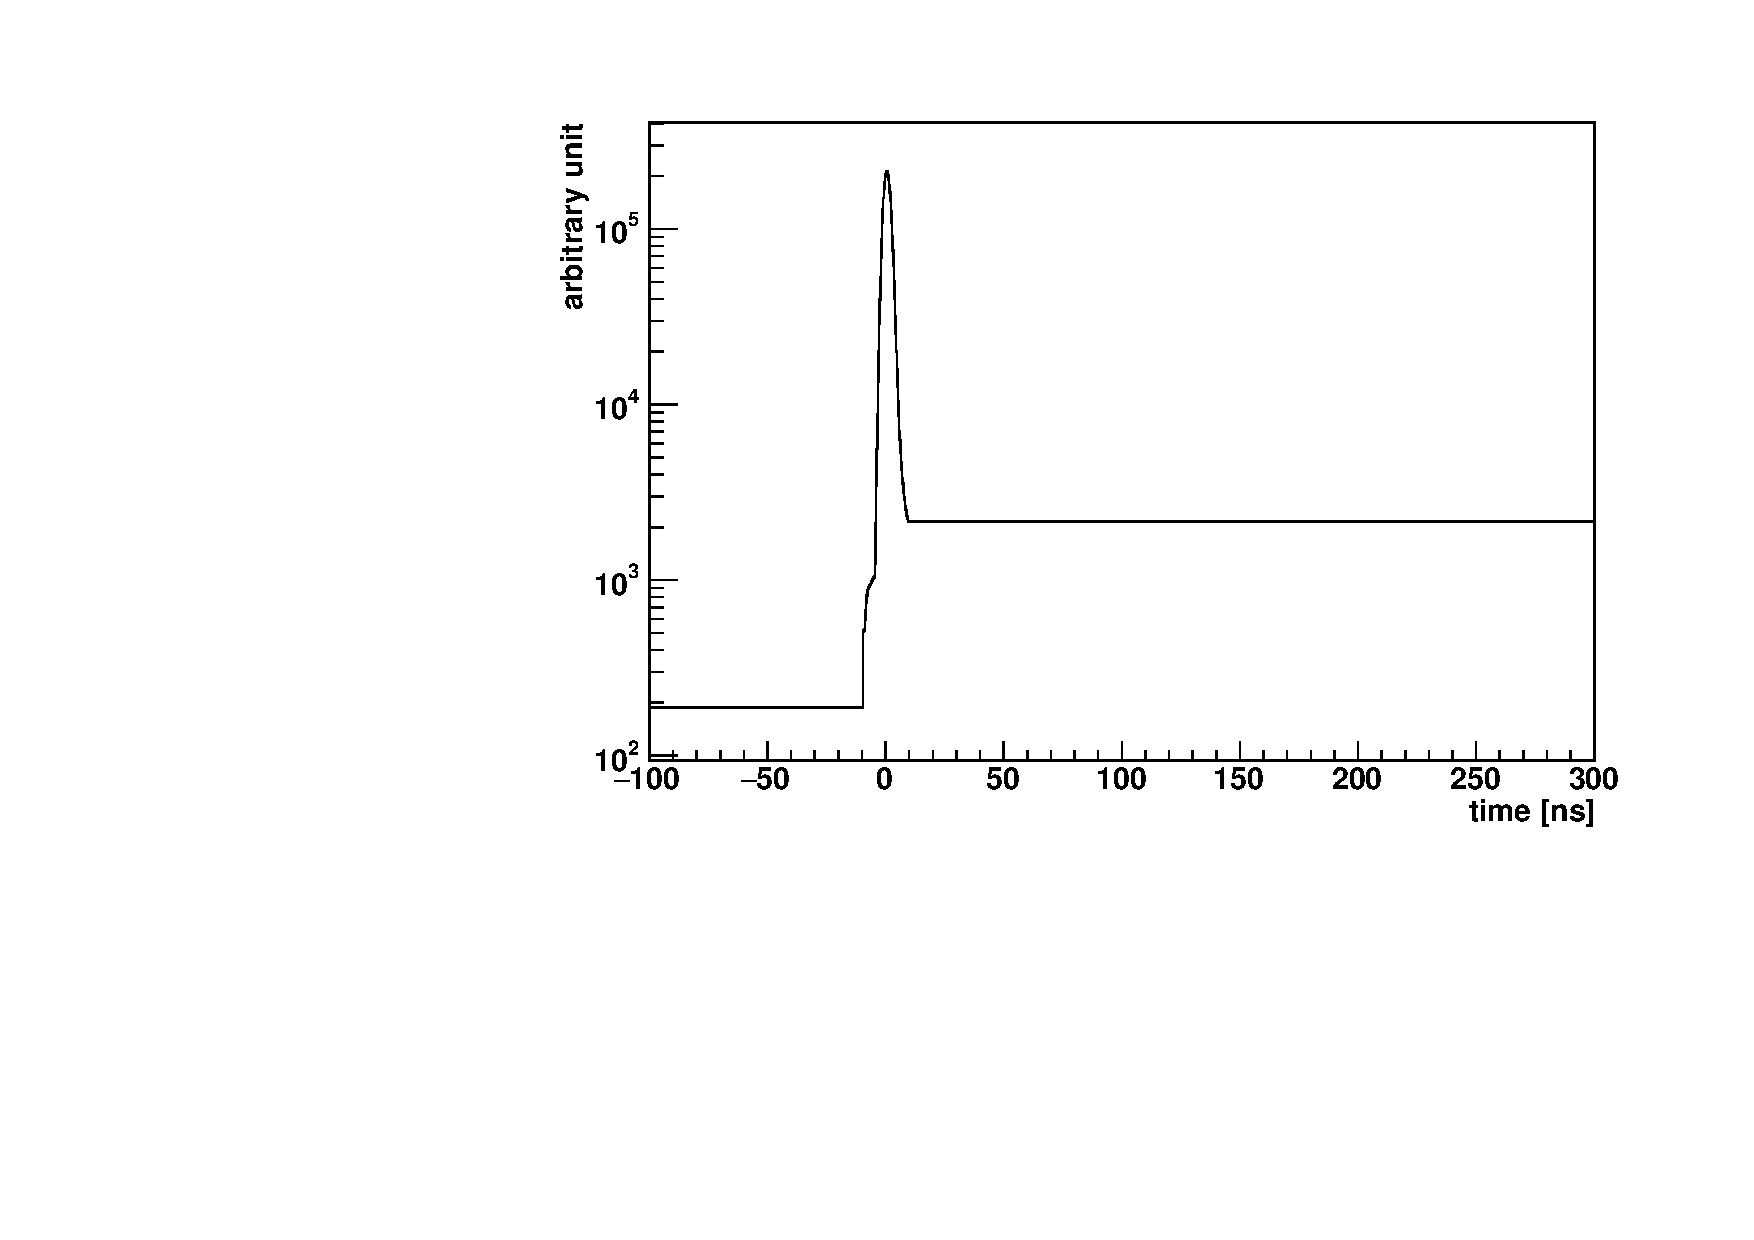
\includegraphics[width=7cm]{MPW_timingPDF.pdf}
	\end{minipage}
	\begin{minipage}[t]{0.48\textwidth}
		\centering
		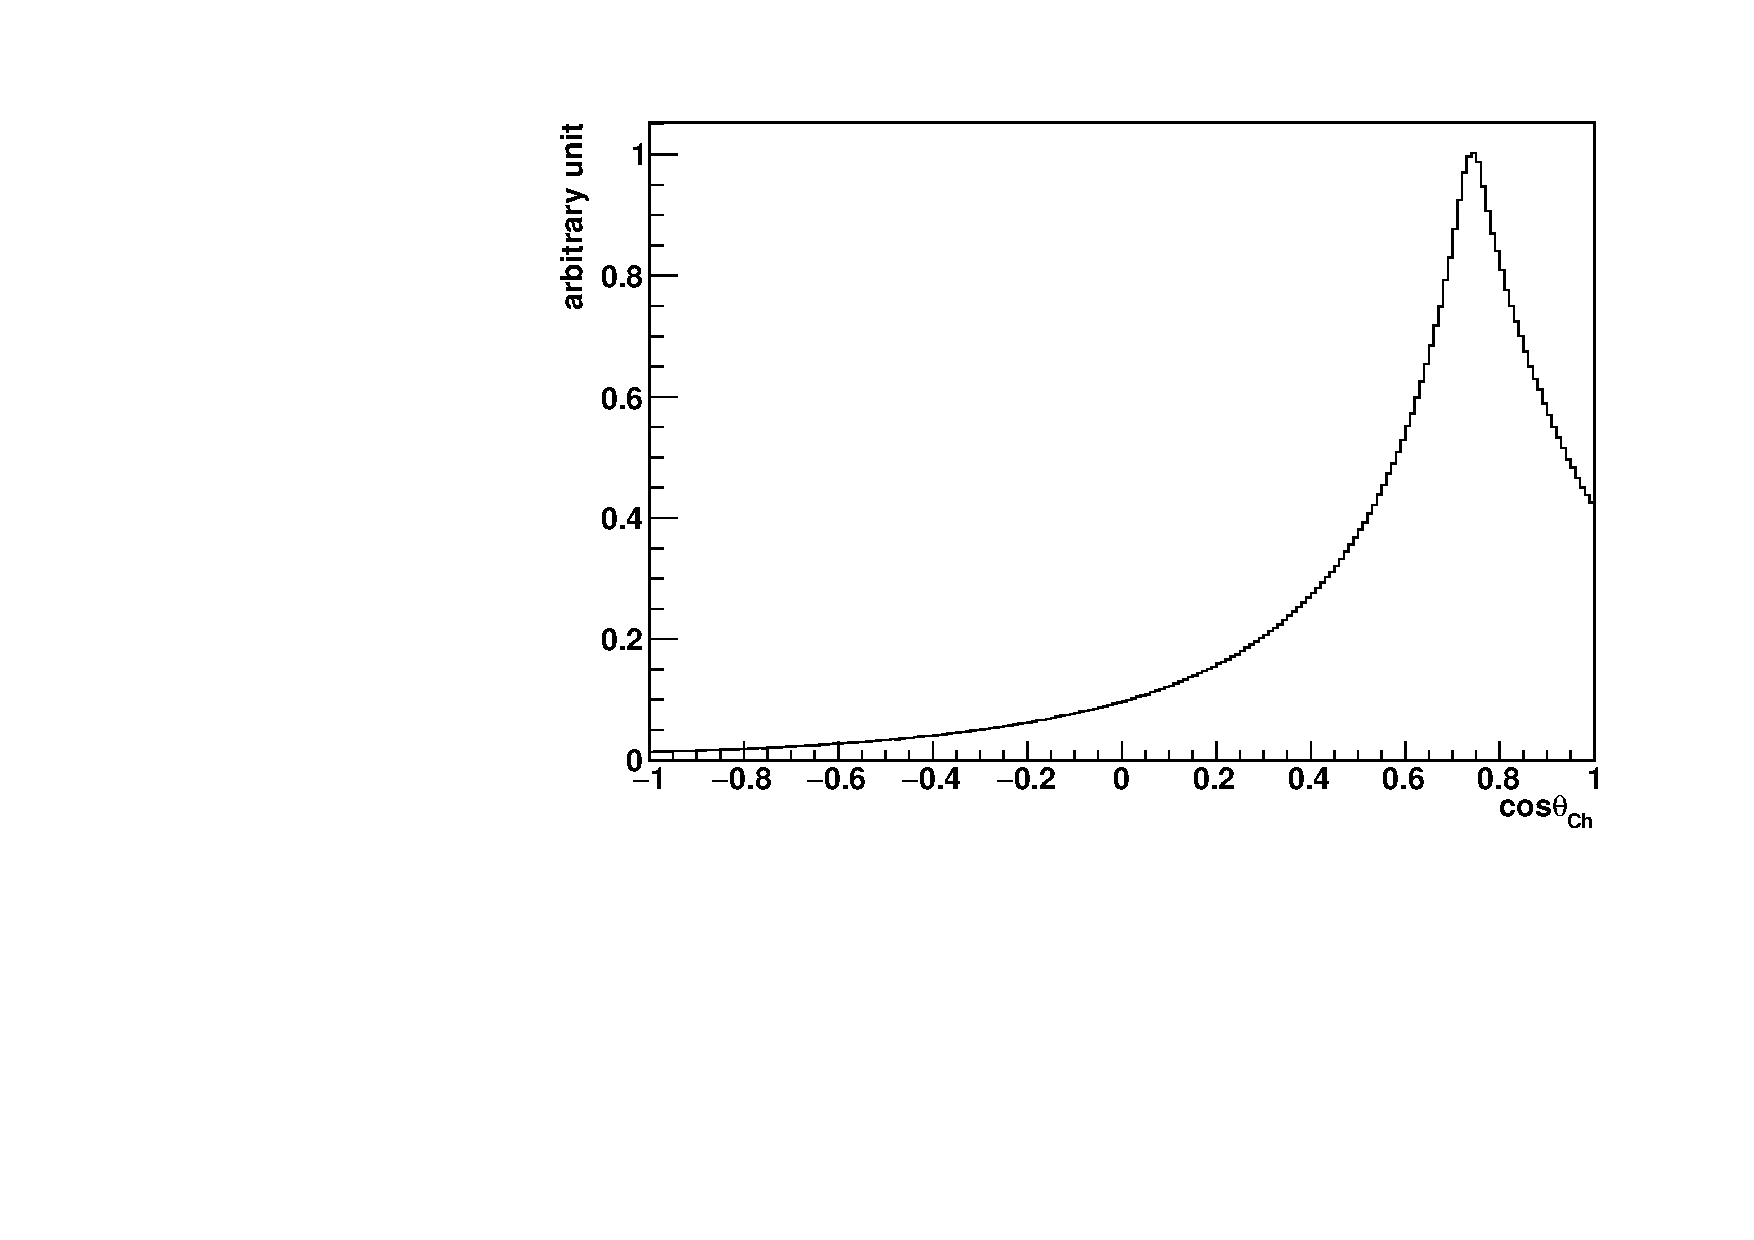
\includegraphics[width=7cm]{MPW_angularPDF.pdf}
	\end{minipage}
	\caption{The pdfs for the MPW fitter. Left: PMT response time tuned by calibration data as the timing pdf. Right: PMT angular distribution as the angular response pdf.}
    \label{mpwpdf}
\end{figure}

\section{Testing the MPW Fitter with SNO+ $^{16}$N Calibration}
The SNO+ detector has been operating in the water phase for a year. In order to calibrate the detector, a $^{16}$N calibration source inherited from the SNO experiment was deployed for calibration scans in June and November, 2017 and March, 2018. 

The $^{16}$N calibration runs provide an ideal test of fitter performance. From a comparison of reconstruction for data and MC, we can also extract the resolution and bias of the MPW fitter. 

\subsection{Fitter Performance}

The $\gamma$ rays emitted from the $^{16}$N source interact with the water in the detector mainly via Compton scattering. Figure~\ref{hsx} shows the spatial distributions of the first $\gamma$-ray interaction points projected on the x axis (called spatial distribution $S(x)$) obtained from MC simulation. The $^{16}$N source is considered as an electron source with a known spatial distribution\cite{boulay}. For simplicity, in the following we always discuss the x component of the position vector $\vec{X}$. 

\begin{figure}[!htb]
	\centering
	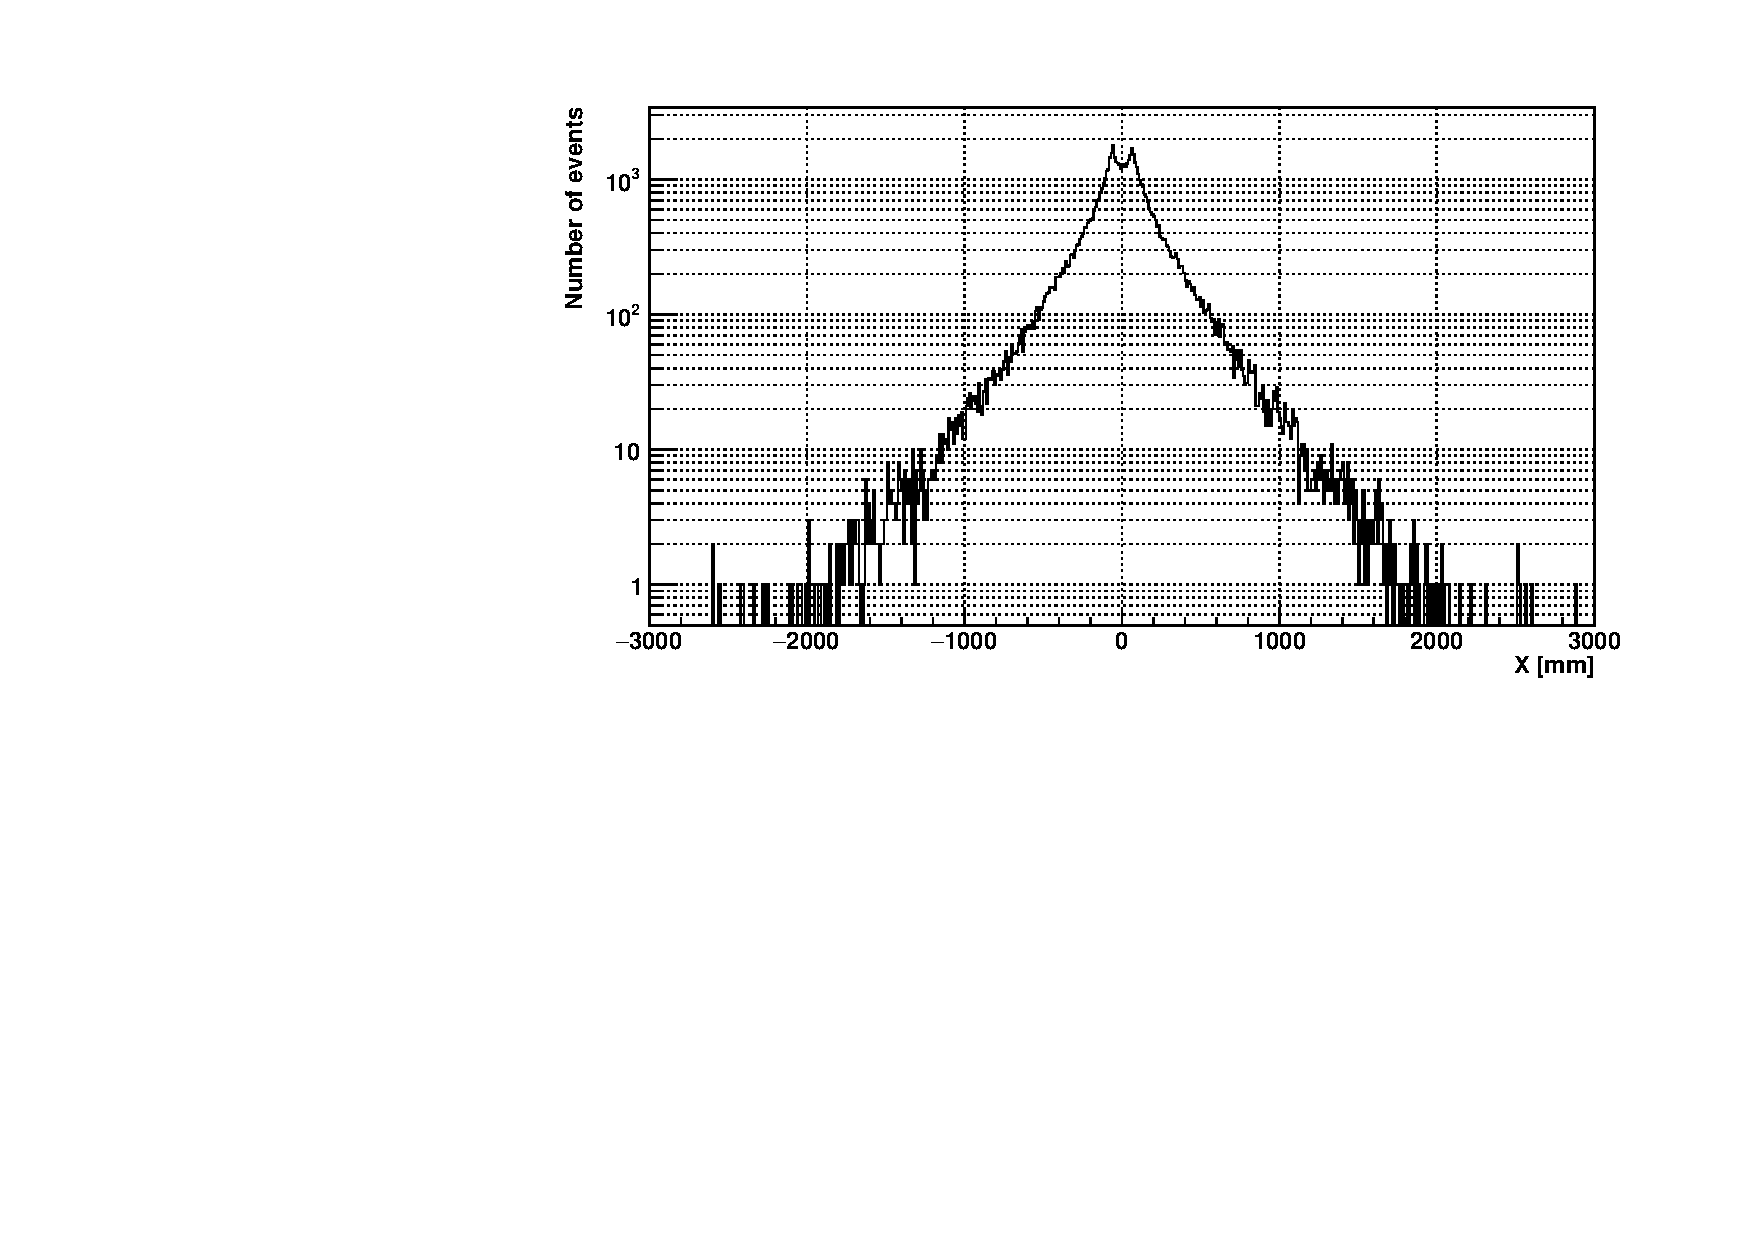
\includegraphics[width=9cm]{sx.pdf}
	\caption{Spatial distributions of {$^{16}$}N first $\gamma$-rays interaction position projected on x axis, obtained from simulations.}
	\label{hsx}
\end{figure}

A position resolution function is defined for the reconstructed electron position distribution\cite{boulay}:
\[
  R(x)=\frac{1-\alpha_e}{\sqrt{2\pi}\sigma_p}\exp{[-\frac{1}{2}(\frac{x-\mu_p}{\sigma_p})^2]+\frac{\alpha_e}{2\tau_p}\exp{[\frac{-|x-\mu_p|}{\tau_p}]}},
\]
where: $\alpha_e$ is the fractional exponential component, $\sigma_p$ is
the Gaussian width, $\mu_p$ is the Gaussian shift and $\tau_p$ is the
exponential slope.

For electrons from the $^{16}$N calibration source, their spatial distribution function $N_{R}(x)$ can be described by the position resolution function smeared by the convolution of $S(x)$ as\cite{boulay}:
\[
  N_{R}(x)=\int^{+\infty}_{-\infty} S(x)R(x_{fit}-x)dx.
\]

Since the $S(x)$ and $N_{R}(x)$ are histograms obtained from the data and MC, we calculate by the bin value $x_i$: 
\[N_R(x_i)=\sum_{x_i=-\infty}^{+\infty}S(x_i)R(x_{fit}^i-x_i).\].

The $\chi^2$ is calculated by:
\[
  \chi^2=\sum^{N_{bins}}_{i=0}[\frac{N_R(x_{fit}^i)-N_R^{fit}(x_{fit}^i)}{\sigma_i}]^2,
\]
where $N_R^{fit}$ is a trial fit to the $N_R$ by tuning the $\{\alpha_e,\mu_p,\sigma_p,\tau_p\}$ and $\sigma_i$ is taken as the bin width of the histograms.

By minimizing the $\chi^2$, the parameters of the resolution function, $\{\alpha_e,\mu_p,\sigma_p,\tau_p\}$ and a best $N_R^{fit}$ are obtained.

Figure~\ref{posresol} shows a comparison of the reconstructed x position of {$^{16}$}N events between data and MC. The reconstructed position distributions are fitted with $N_R^{fit}$.

\begin{figure}[!htb]
	\centering
	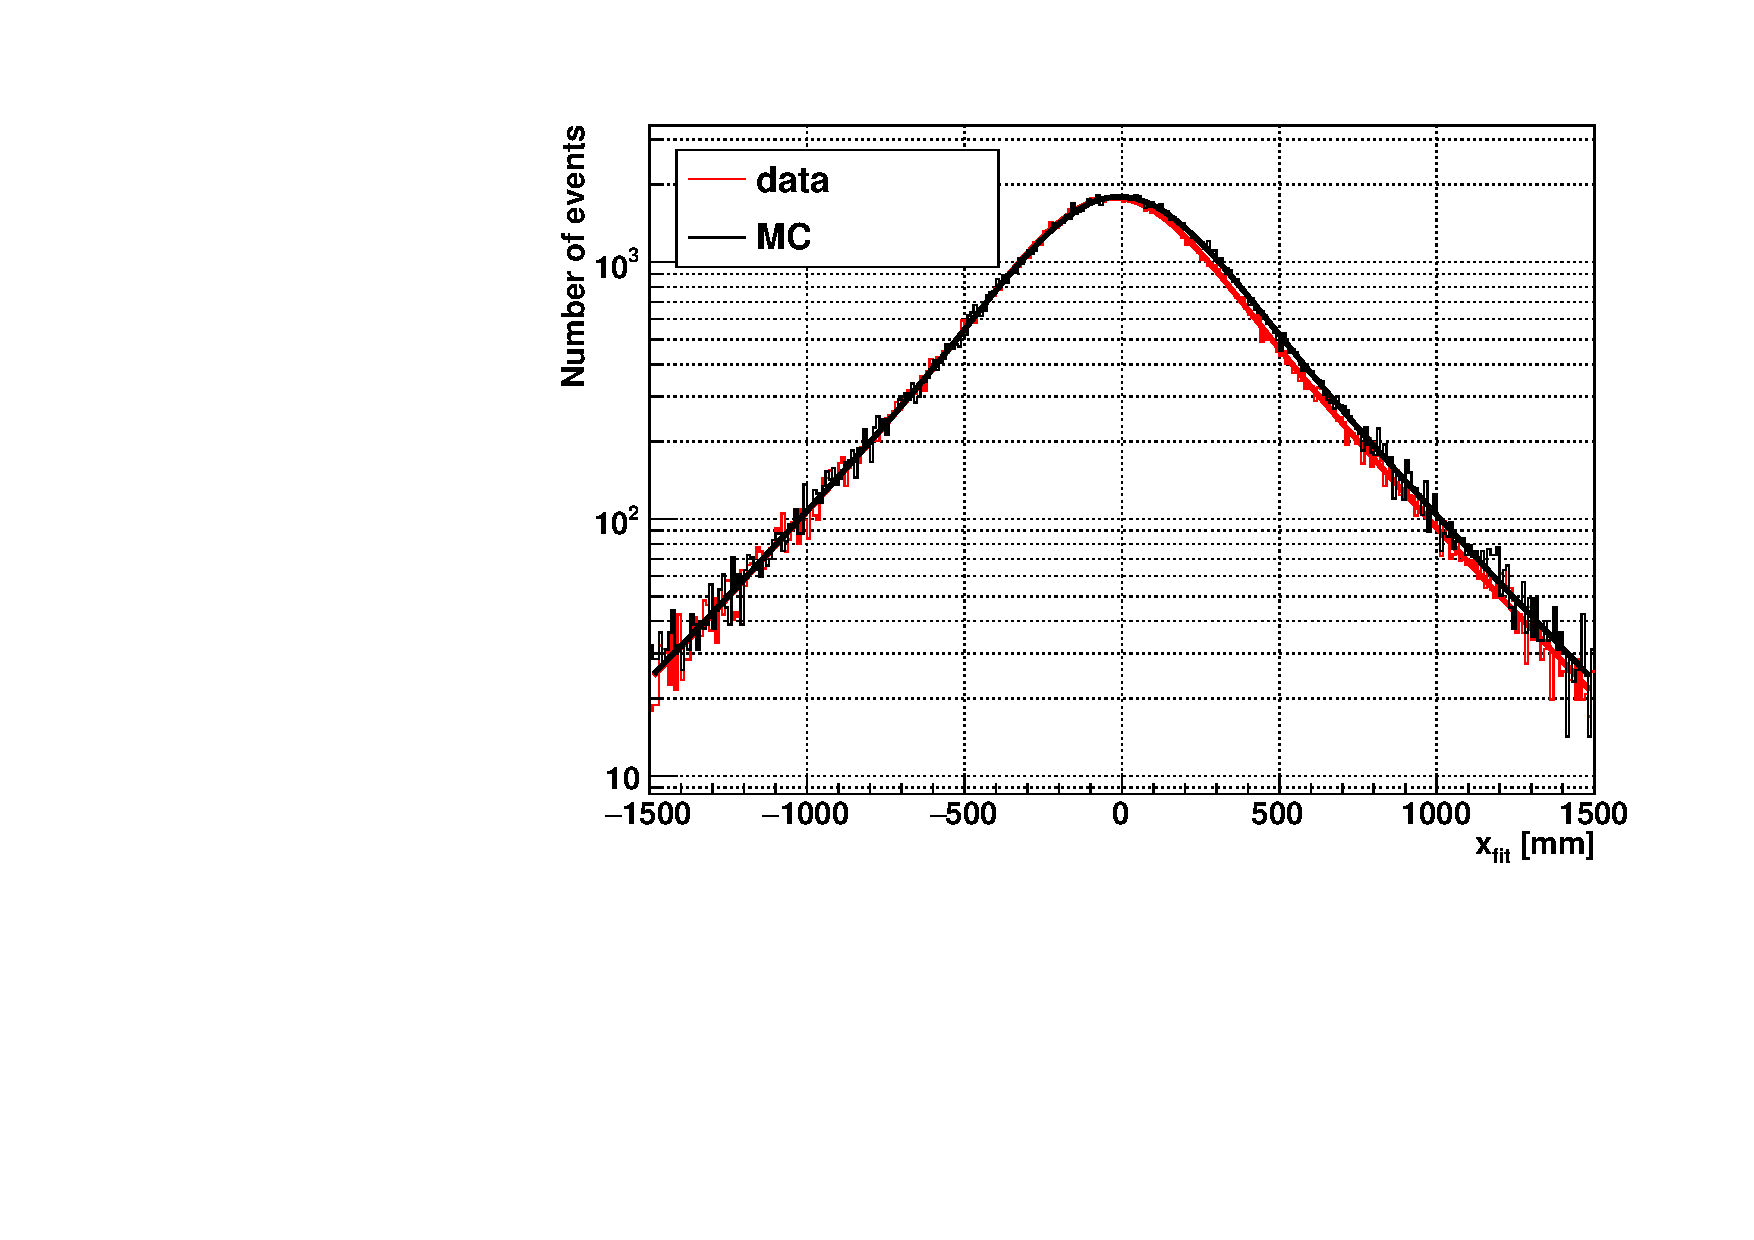
\includegraphics[width=10cm]{posResol.pdf}
	\caption{Distributions of the reconstructed position projected on x axis, obtained from SNO+ {$^{16}$}N central run data (red) and MC (black). The distributions are fitted with $N_R^{fit}$ (red and black lines), the position resolution function convolved with the distribution of the first $\gamma$ interaction positions.}
	\label{posresol}
\end{figure}

Table~\ref{table_posresol} summarizes the values of position biases and resolutions obtained from data and MC of {$^{16}$}N calibration runs at the detector center.
\vspace{1mm}
\begin{table}[ht]
\centering
\caption{Position resolution parameters for the MPW fitter.}
\label{table_posresol}
\begin{tabular}{|p{2.5cm}|p{2.2cm}|p{2.1cm}|p{2.1cm}|p{2.1cm}| p{2.1cm}|}
\hline
MPW fitter & $\alpha_e$ & $\sigma_P$ (mm) &  $\tau_P$ (mm)& $\mu_P$ (mm)\\
\hline 
data& 0.58$\pm$0.04 & 175.8$\pm$3.8 & 288.0$\pm$5.7 & -28.8$\pm$1.0\\	
\hline 
MC & 0.51$\pm$0.05 & 195.2$\pm$3.3 & 298.4$\pm$6.1 & -10.9$\pm$1.0\\
\hline
\end{tabular}
\end{table}
\vspace{1mm}

\section{SNO+ Partial-fill Reconstruction}
\subsection{MultiPath Partial Fitter}
In the same MP fitter framework, a MP partial fitter is developed for SNO+ partial-fill position and time reconstruction.

In the partial fill geometry, photons will travel with different speeds as they pass through two different mediums, water and scintillator. Assuming a straight light path, the MP partial fitter mainly calculates the total length of the light path ($|\vec{l}_p|=|\vec{X}_{PMT}-\vec{X}_{vertex}|$) and separates it into the lengths in scintillator ($d_{sp}$) and in water ($|\vec{l}_p|-d_{sp}$).

\begin{figure}[!htb]
	\centering
	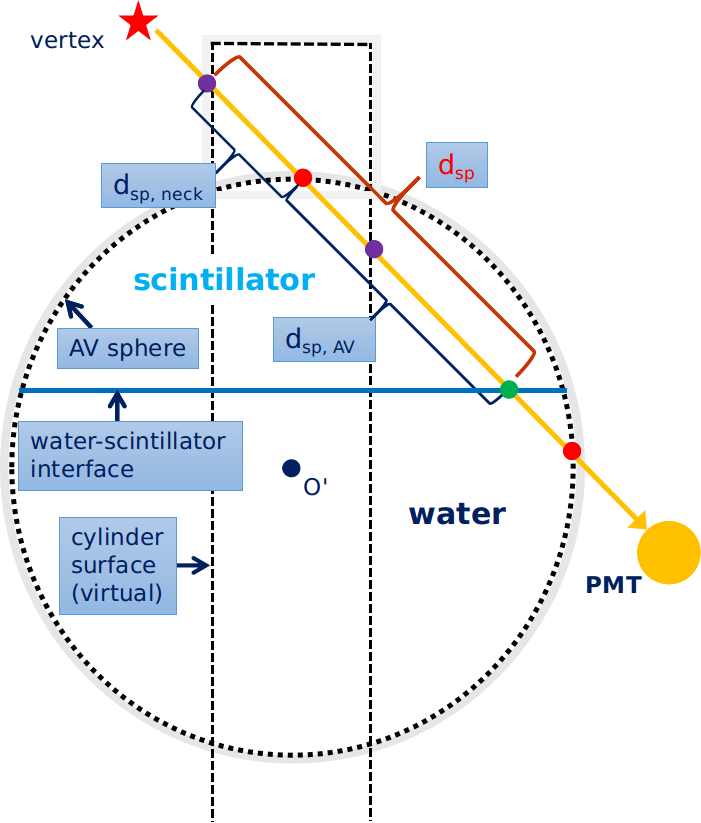
\includegraphics[width=7cm]{scintpath.png}
	\caption{Light path calculation for the partial fitter.}
	\label{scintpath}
\end{figure}

As illustrated in Figure~\ref{scintpath}, a detailed calculation of $d_{sp}$ includes evaluations of (1) light path and neck (line-cylinder) intersection; (2) light path and AV sphere (line-sphere) intersection and (3) light path and water-scintillator interface (line-plane) intersection. $d_{sp}$ is further separated into the path length in neck ($d_{sp,neck}$) and in AV ($d_{sp,AV}$).

Then the time of flight is obtained by:
\begin{equation}
tof = \frac{|\vec{l}_p|-d_{sp}}{v_{gr,water}} +\frac{d_{sp}}{v_{gr,scint}},
\end{equation}
The time residual is $t_{res} = t_{PMT}-tof-t_0$.

\begin{figure}[htbp]
	\centering	
	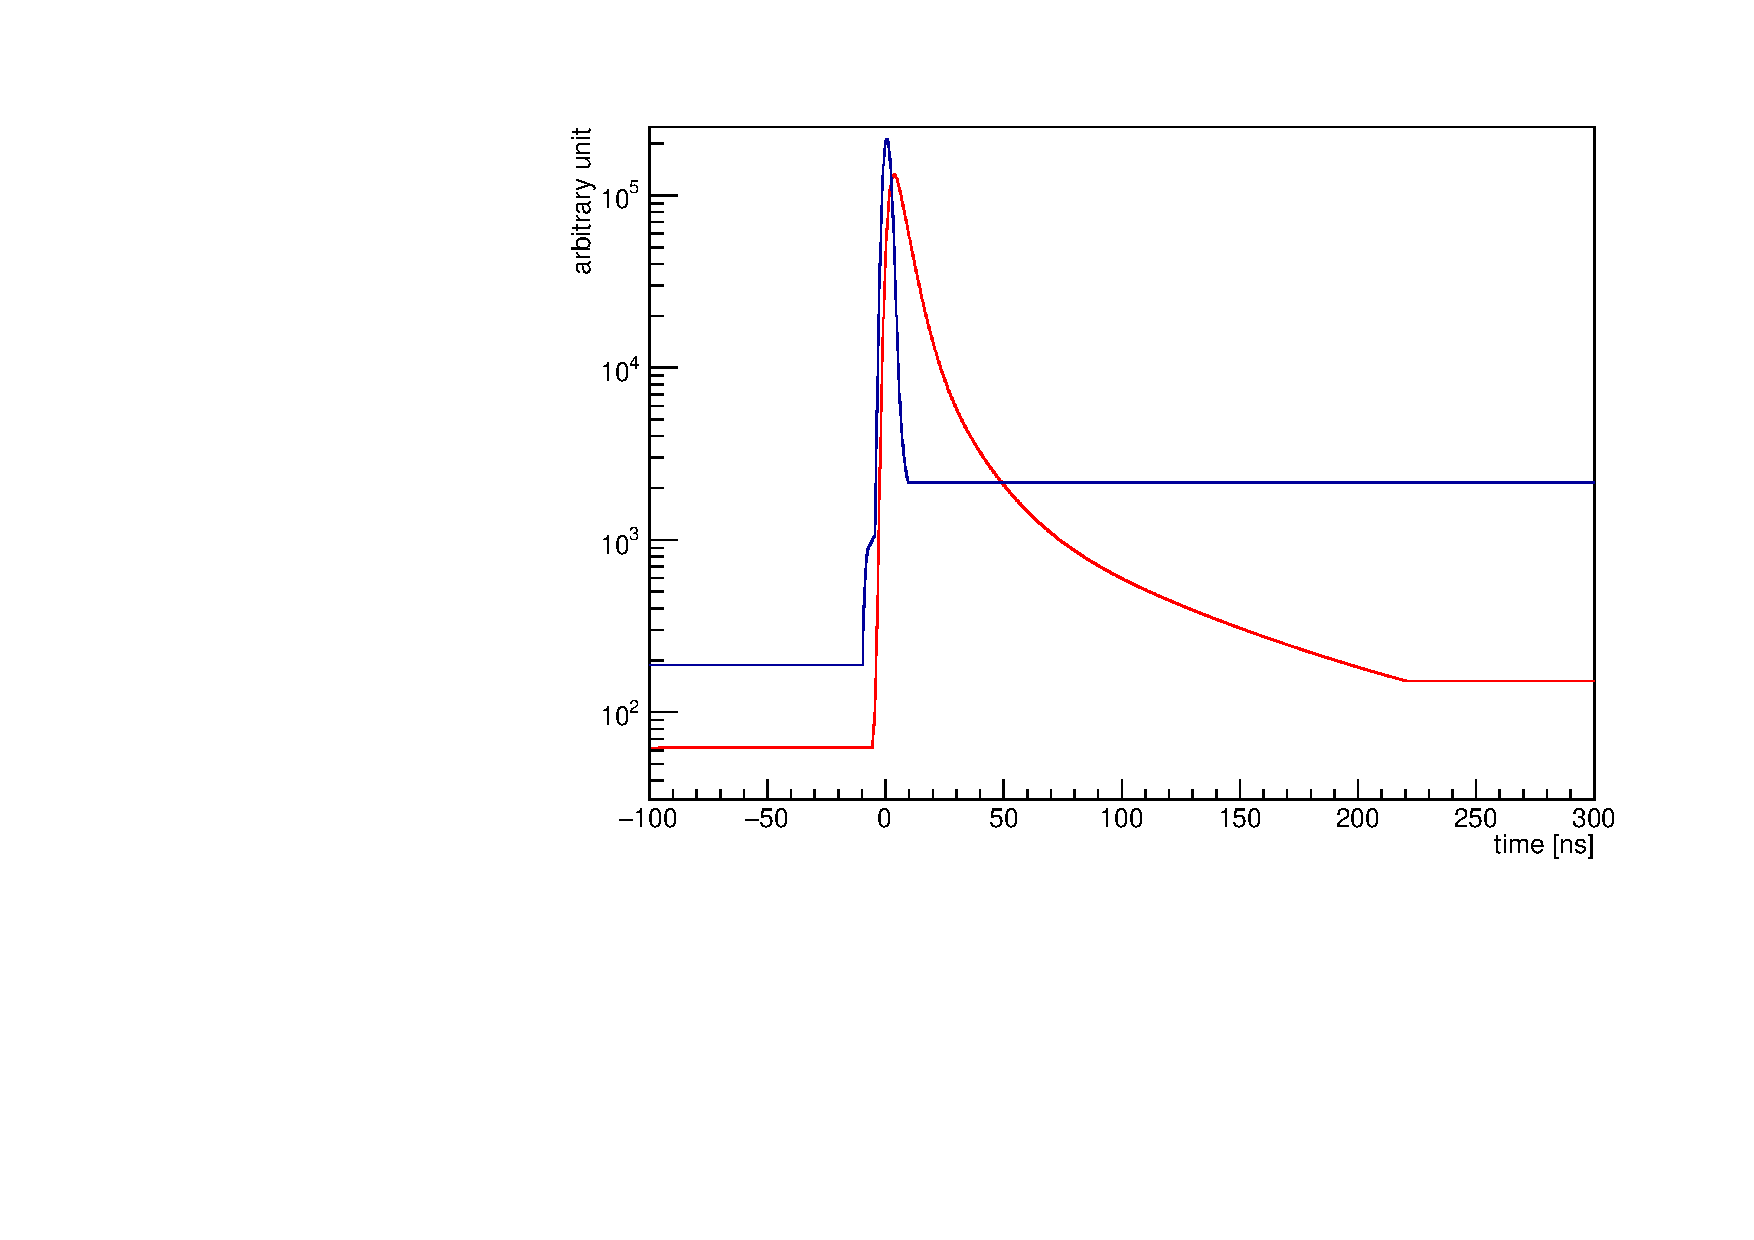
\includegraphics[width=7cm]{scintpdf.pdf}
	\caption{The pdfs used by MP partial fitter. Blue: the timing pdf used by the MPW fitter; Red: the scintillator timing pdf.}
	\label{partialpdf}
\end{figure}

If $d_{sp}=0$, the light path is always in the water. In this case, the fitter is the same as the MPW. The fitter fits with the MPW pdf. Once the light path passes through the scintillator region, the fitter fits with a scintillator timing pdf, as shown in Figure~\ref{partialpdf}.

\begin{figure}[htbp]
	\centering
	\subfloat[scintillator region]{
		\begin{minipage}[t]{0.38\textwidth}
			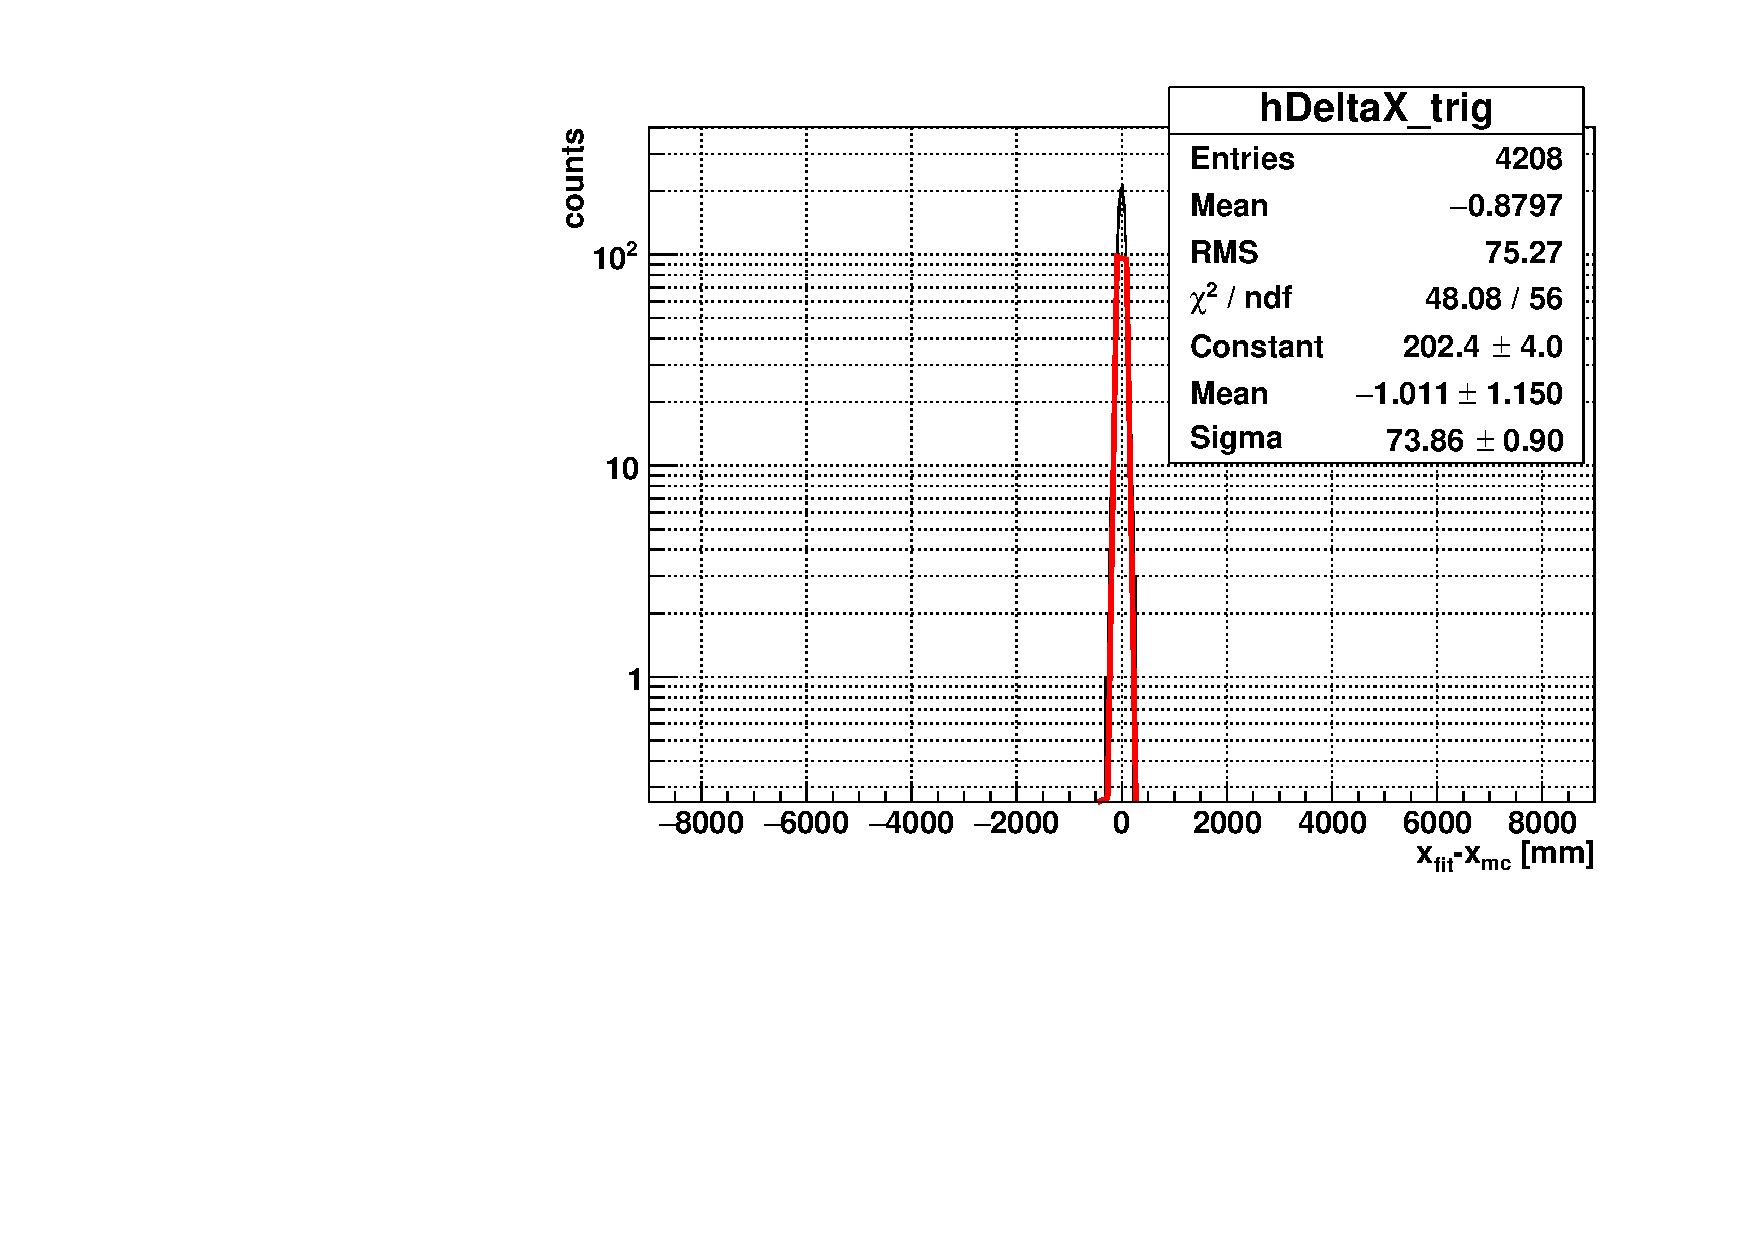
\includegraphics[width=6cm]{partial_top_x.pdf}
		\end{minipage}
	}   
	\subfloat[water region]{ 
		\begin{minipage}[t]{0.38\textwidth}
			\centering
			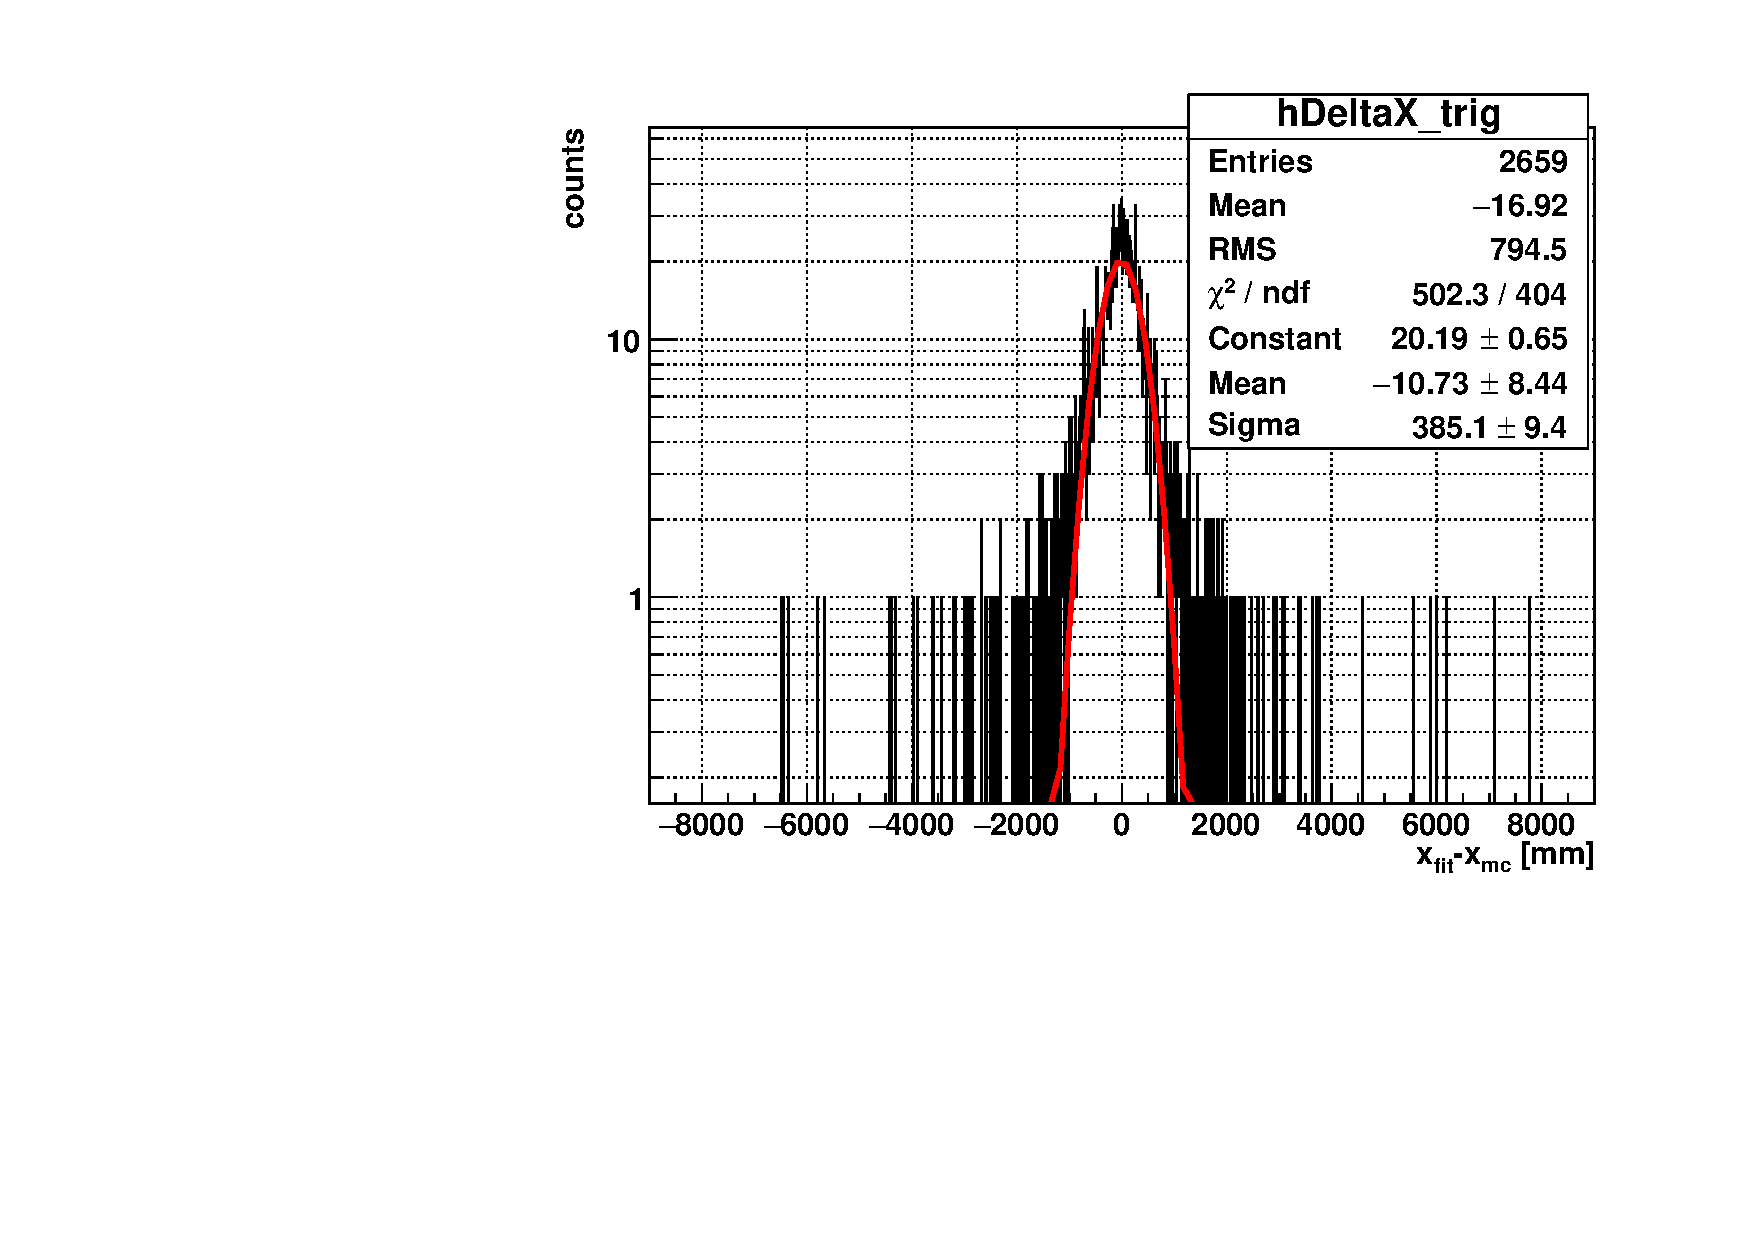
\includegraphics[width=6cm]{partial_bot_x.pdf}
		\end{minipage}
	}
	\subfloat[whole region]{ 
		\begin{minipage}[b]{0.32\textwidth}
			\centering
			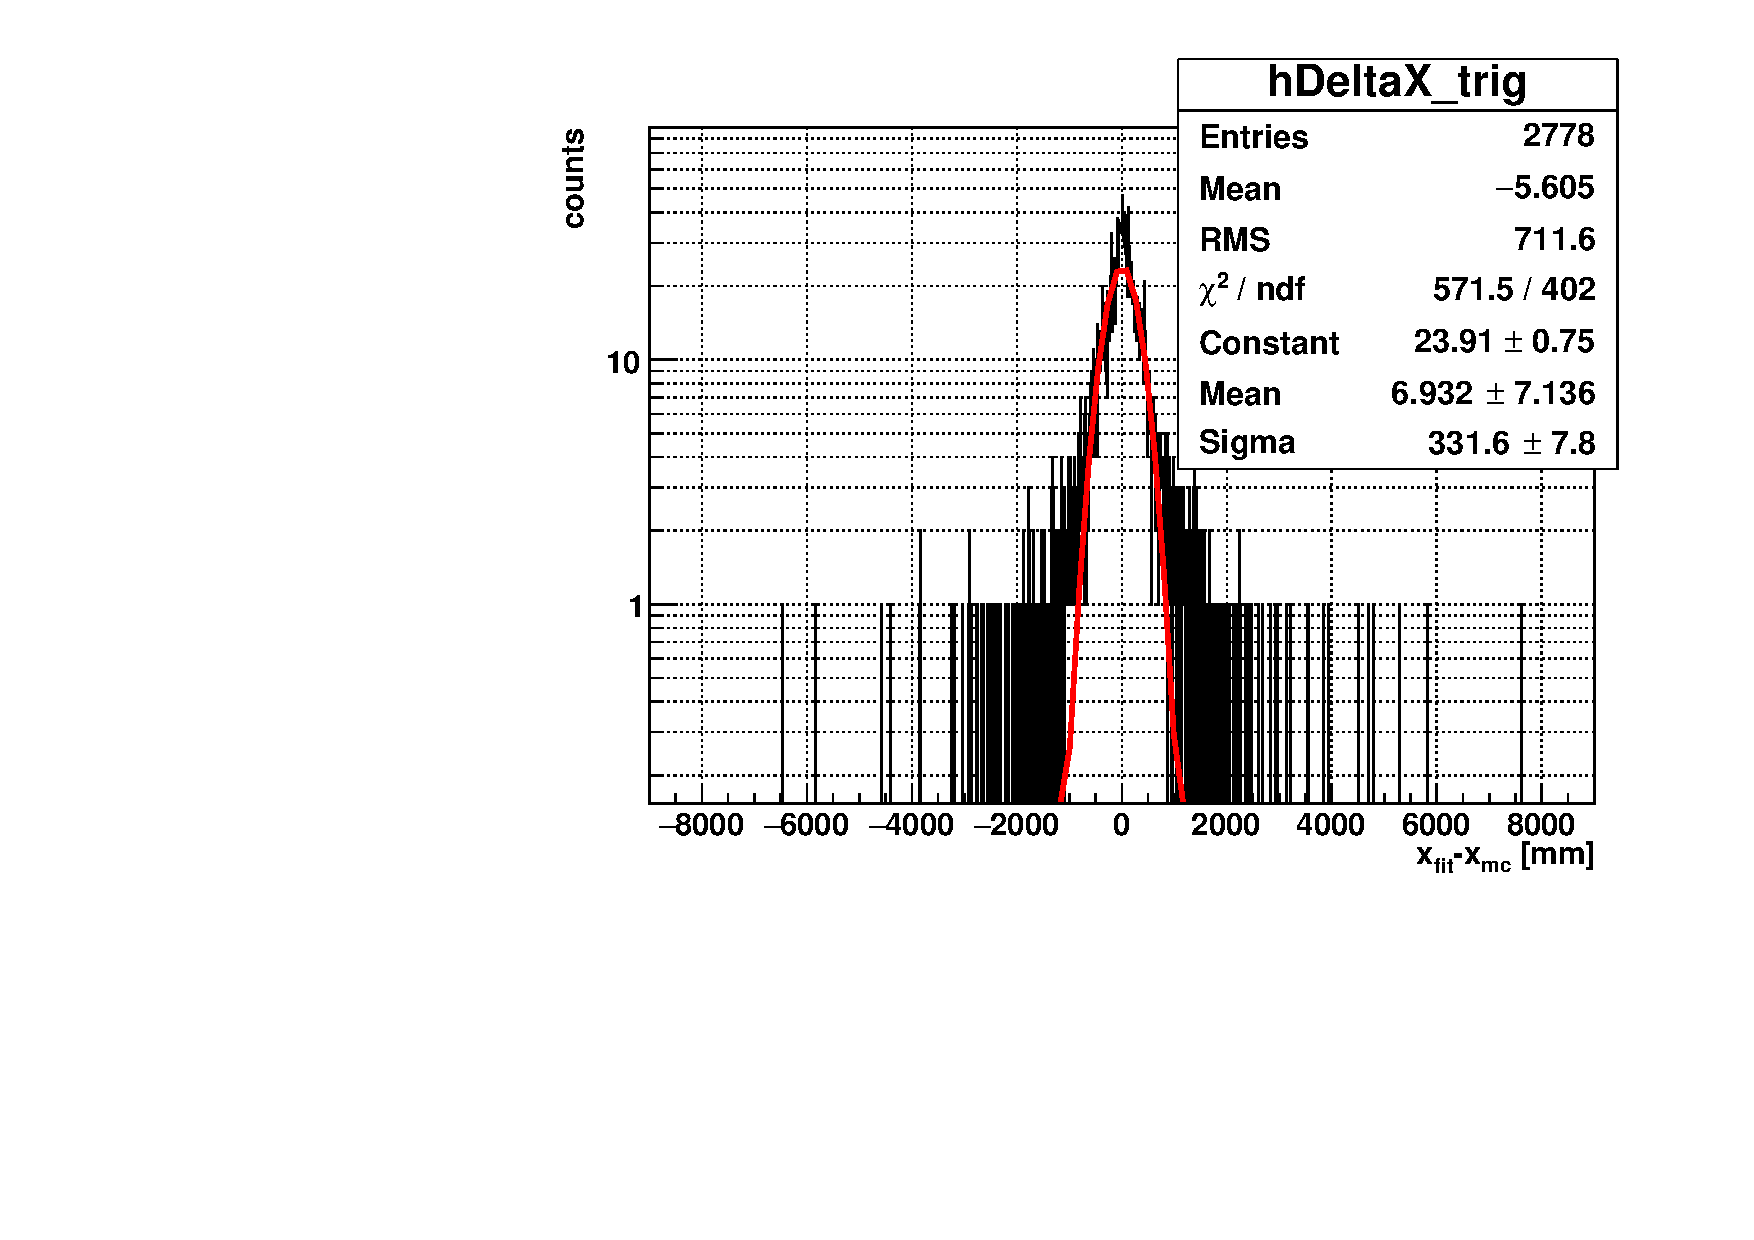
\includegraphics[width=6cm]{partial_full_x.pdf}
		\end{minipage}
	}
	\caption{Distributions of fit position bias projected on x axis ($x_{fit}-x_{MC}$).}
	\label{partial_fit_x}
	\subfloat[scintillator region]{ 
		\begin{minipage}[t]{0.38\textwidth}
			\centering
			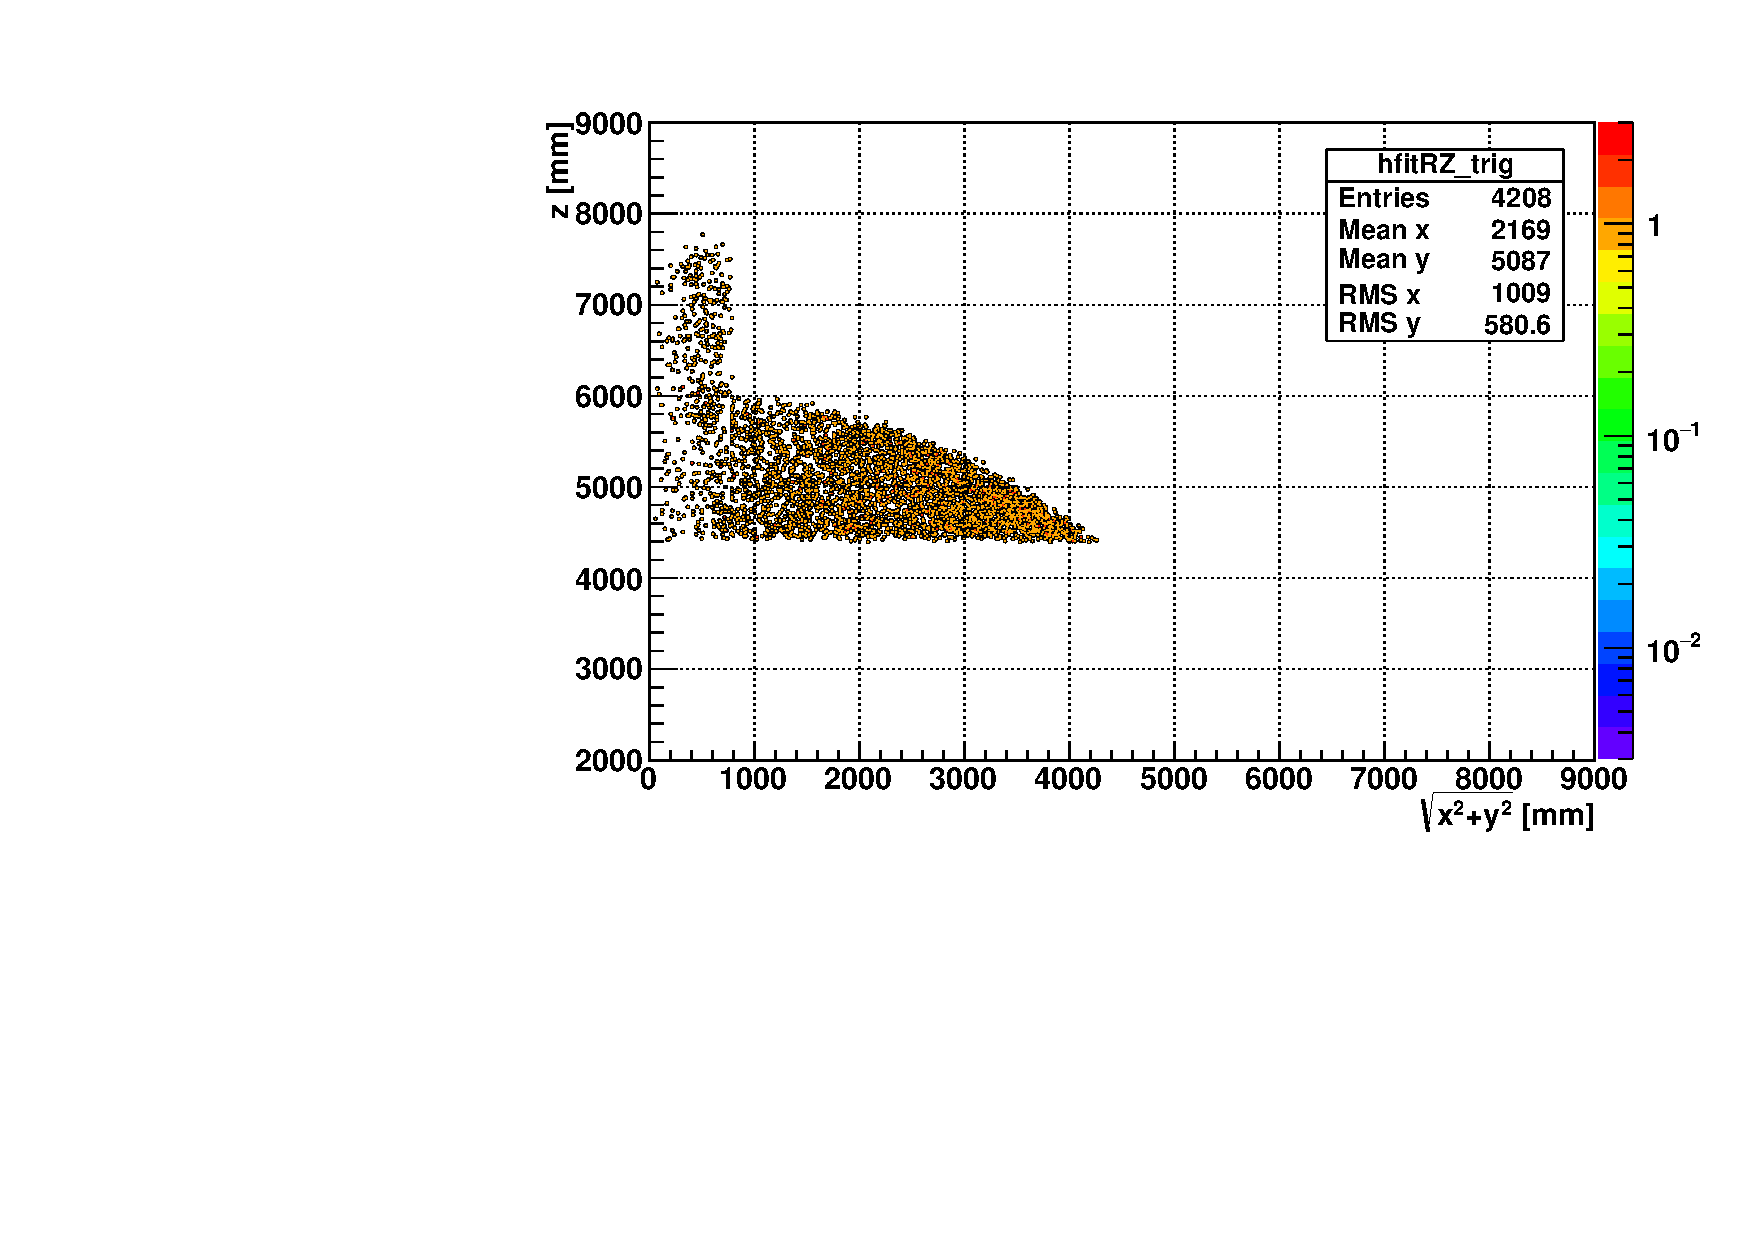
\includegraphics[width=5.8cm]{partial_top_r.pdf}
		\end{minipage}
	}
	\subfloat[water region]{ 
		\begin{minipage}[t]{0.38\textwidth}
			\centering
			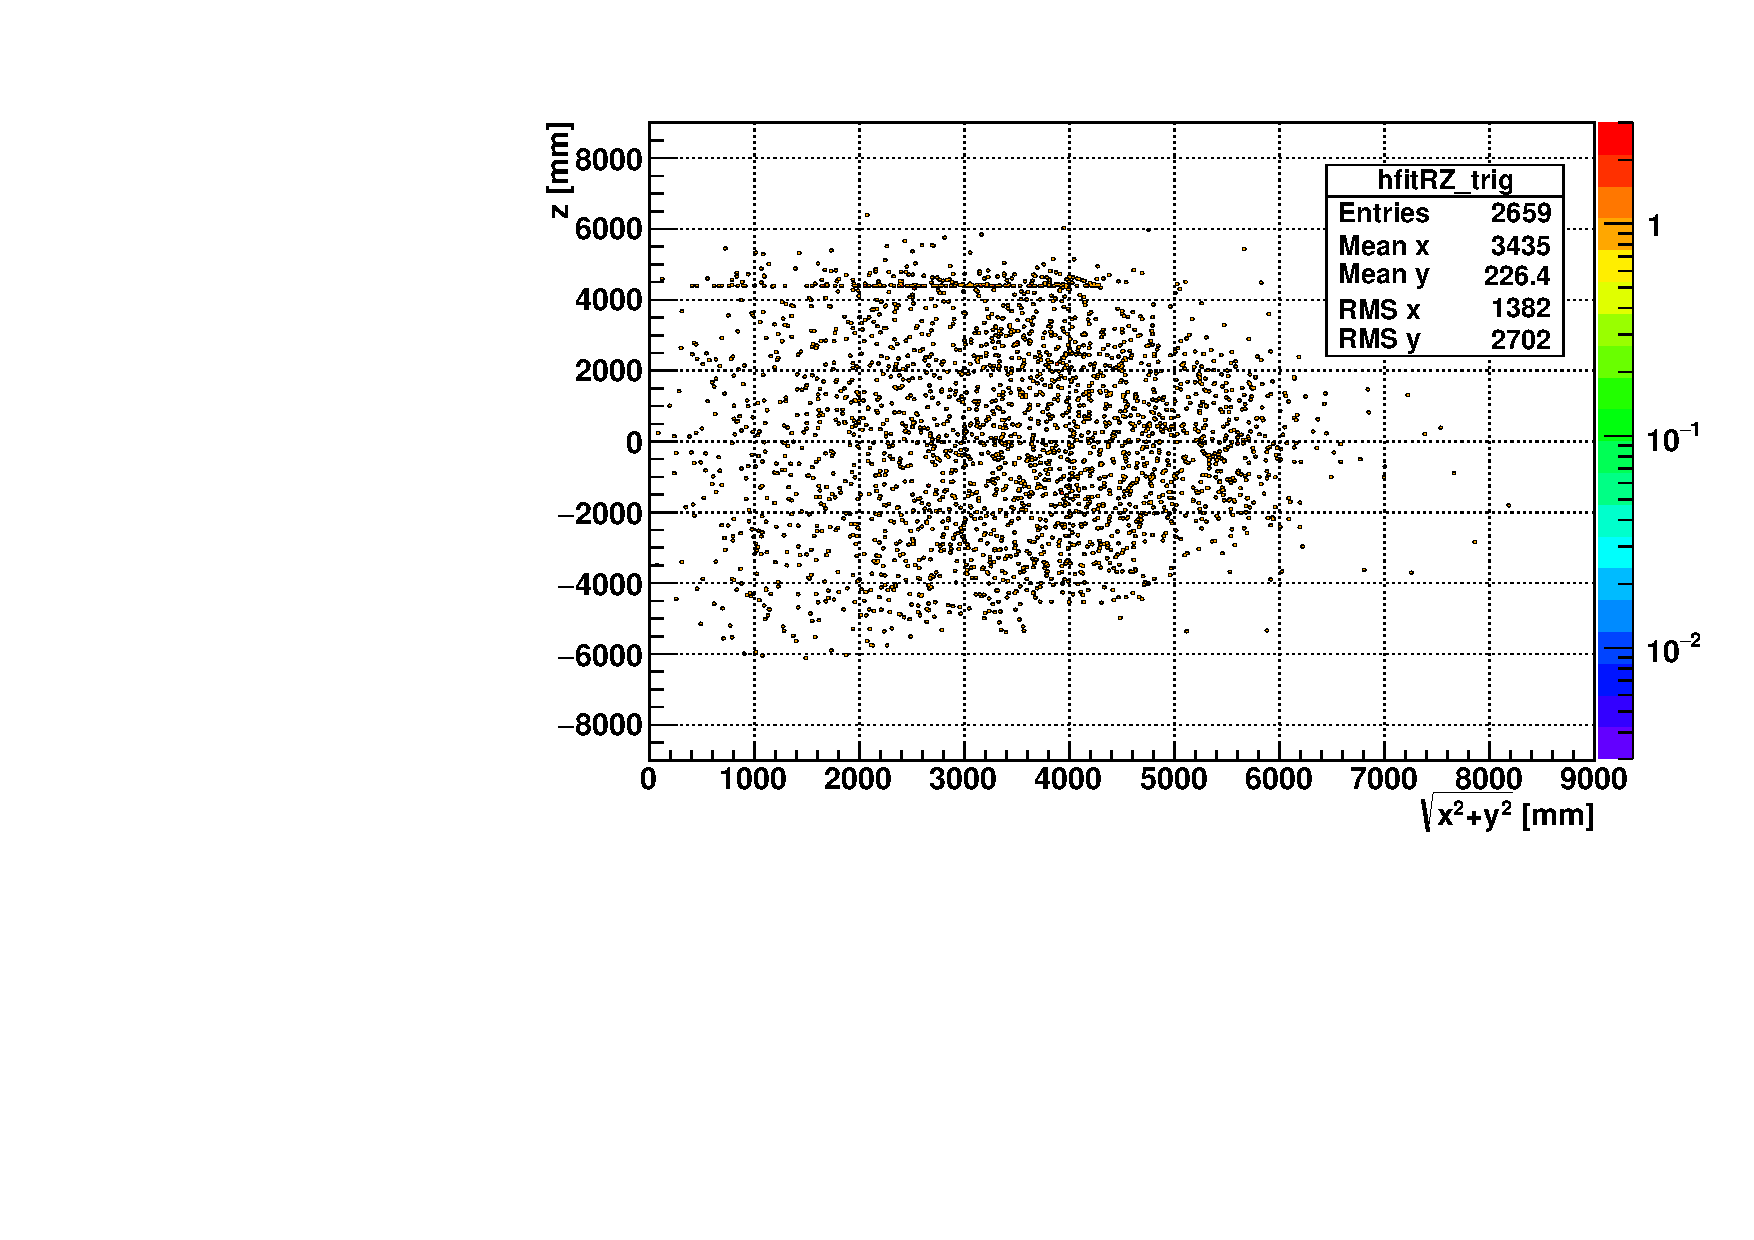
\includegraphics[width=5.8cm]{partial_bot_r.pdf}
		\end{minipage}
	}
	\subfloat[whole region]{ 
		\begin{minipage}[b]{0.35\textwidth}
			\centering
			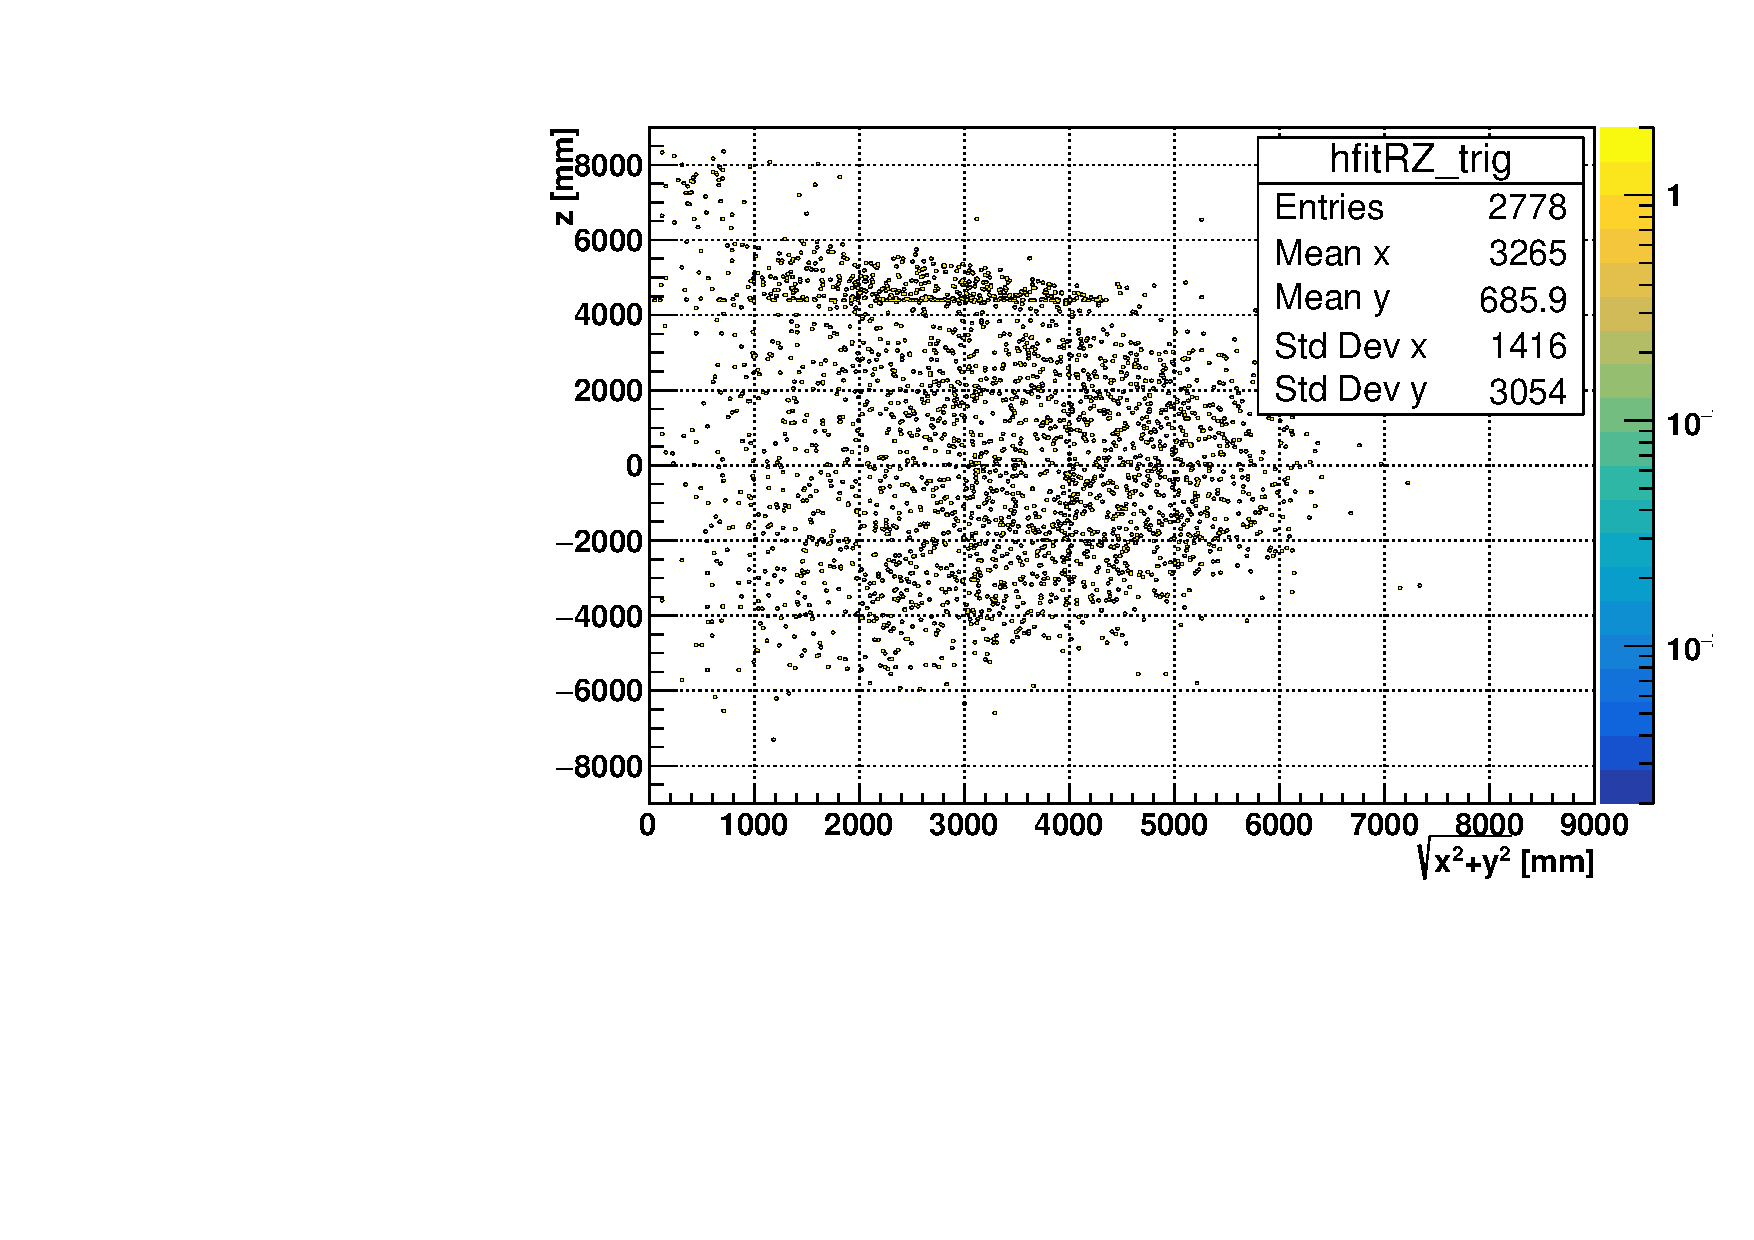
\includegraphics[width=5.8cm]{partial_full_r.pdf}
		\end{minipage}
	}
	\caption{Fit results: $\rho_{fit}=\sqrt{x_{fit}^2+y_{fit}^2}$ vs. $z_{fit}$.}
	\label{partial_fit_rz}
\end{figure}

The performance of the fitter was studied with MC simulations. In a partial fill geometry with water level at 4.4 m, 2.5 MeV electrons are simulated inside the AV in the scintillator region only, the water region only and the whole AV region.

Figure~\ref{partial_fit_x} and Figure~\ref{partial_fit_rz} show the MP Partial fitter reconstructed results for these simulations. Figure~\ref{partial_fit_x} shows the biases between the fit positions and MC positions, projected on the x axis. The distributions of position biases are fit with Gaussian functions. The values of Gaussian mean and sigma quantify the fit biases and resolutions. Table~\ref{partiaResol} lists these values.

\begin{table}[ht]
	\centering
	\caption{Reconstructed position biases and resolutions for simulated events in partial fill.}
	\label{partiaResol}
	\begin{tabular*}{120mm}{c@{\extracolsep{\fill}}ccc}
		\hline
		regions of simulated events& bias (mm) &  resolution (mm) \\
		\hline
		scintillator region & -1.0  & 73.9\\
		water region & -10.7 & 385.1\\
		full region &6.9 & 331.72\\
		\hline
	\end{tabular*}
\end{table}
For the events in water, the fit bias and resolution is comparable to the water phase results in Table~\ref{table_posresol}. The events in the scintillator region have smaller fit bias and better resolution due to more triggered PMTs in the reconstruction.

Figure~\ref{partial_fit_rz} shows the fit $\sqrt{x^2+y^2}$ vs. fit z positions. It shows that the fitter can distinguish different events in the water or scintillator region. The fitter gives reasonable results of the three different MC simulations. 

\section{Thesis Research Plan}
October to November, 2018: My work is focusing on the further development of the reconstruction algorithm related to the partial fill and scintillator phases. The accuracy and speed of the partial fitter are being improved. The fitter will be tested on MC simulations of backgrounds. Based on the reconstructed results of the simulations, the methods of event classification as well as the cuts for distinguishing signals from backgrounds will be developed.

November, 2018 to Spring, 2019: In this period, I will analyze the partial fill data and the scintillator phase data with the reconstruction algorithms I am developing. The analyses will focus on an understanding of the backgrounds and searching for solar neutrino signals. $^{238}$U is one of the natural radioisotopes found in the scintillator\cite{stefanie_thesis}. It goes through a series of radioactive decays, called decay chain, which produces different radioisotopes. These radioisotopes may mimic the solar neutrino signals. One focus of the background analysis is to determine the level of $^{238}$U in the scintillator. The solar neutrino analysis will focus on the methods of signal extraction and the evaluations of solar neutrino events.

I will start writing my thesis in summer, 2019.

\vspace{30mm}
\bibliographystyle{elsarticle-num}

\begin{thebibliography}{00}
\bibitem{wiki_nu} \url{https://en.wikipedia.org/wiki/Neutrino}	

\bibitem{cowanexpintro} Anderson, E.C. The Reines-Cowan Experiments. 

\url{http://permalink.lanl.gov/object/tr?what=info:lanl-repo/lareport/LA-UR-97-2534-02}
\bibitem{bethe1} H. Bethe and R. Peierls. The `neutrino'. Nature, 133:5321934.

\bibitem{hyperphysicsCowan} \url{http://hyperphysics.phy-astr.gsu.edu/hbase/Particles/cowan.html}

\bibitem{bethe2} Bethe, Hans Albrecht. ``Energy production in stars." Physical Review 55.5 (1939): 434.

\bibitem{oxfordneutrino} Giunti, Carlo, and Chung W. Kim. Fundamentals of neutrino physics and astrophysics. Oxford university press, 2007.

\bibitem{haxton_solar} W. C. Haxton et al. ``Solar neutrinos: status and prospects.'' Ann. Rev. Astron. Astrophys., 51:21, 2013

\bibitem{BP05} Bahcall, John N., Aldo M. Serenelli, and Sarbani Basu. ``New solar opacities, abundances, helioseismology, and neutrino fluxes.'' The Astrophysical Journal Letters 621.1 (2005): L85.


\bibitem{bahcall1} Bahcall, John N. ``Solar neutrinos. i. theoretical." Physical Review Letters 12.11 (1964): 300.
\bibitem{raymond} Davis Jr, Raymond. ``Solar neutrinos. ii. experimental." Physical Review Letters 12.11 (1964): 303.

\bibitem{bahcall2} Bahcall, John N. ``Gallium solar neutrino experiments: Absorption cross sections, neutrino spectra, and predicted event rates." Physical Review C 56.6 (1997): 3391.

\bibitem{imb} Becker-Szendy, R., Bratton, C.B., Casper, D., Dye, S.T., Gajewski, W., Goldhaber, M. et al. (1992) Electron- and muon-neutrino content of the atmospheric flux. Phys. Rev. D 46, 3720-3724.

\bibitem{soudan2} Allison, W.W.M., Alner, G.J., Ayres, D.S., Barrett, W.L., Bode, C., Border, P.M. et al. (Soudan-2 collaboration) (1997) Measurement of the atmospheric neutrino flavour composition in Soudan 2. Phys. Lett. B 391, 491-500.

\bibitem{atmNuReview} Takaaki Kajita, ``Atmospheric Neutrinos," Advances in High Energy Physics, vol. 2012, Article ID 504715, 24 pages, 2012. doi:10.1155/2012/504715

\bibitem{herbertChen} Chen, Herbert H. ``Direct approach to resolve the solar-neutrino problem." Physical Review Letters 55.14 (1985): 1534.

\bibitem{SNO} Ahmad, Q. Retal, et al. ``Direct evidence for neutrino flavor transformation from neutral-current interactions in the Sudbury Neutrino Observatory." Physical review letters 89.1 (2002): 011301.

\bibitem{SNOresult} Aharmim, B., et al. ``Combined analysis of all three phases of solar neutrino data from the Sudbury Neutrino Observatory." Physical Review C 88.2 (2013): 025501.

\bibitem{superK} Fukuda, Y., et al. ``Evidence for oscillation of atmospheric neutrinos." Physical Review Letters 81.8 (1998): 1562.

\bibitem{nobeldoc} ``The Nobel Prize in Physics 2015". Nobelprize.org. Nobel Media AB 2014. Web. 1 Oct 2017. \url{http://www.nobelprize.org/nobel_prizes/physics/laureates/2015/}

\bibitem{cahn} Cahn, Robert N., and Gerson Goldhaber. The experimental foundations of particle physics. Cambridge University Press, 2009.

\bibitem{smirnov} Smirnov, A. Yu. ``Solar neutrinos: Oscillations or No-oscillations?." arXiv preprint arXiv:1609.02386 (2016).

\bibitem{smirnov_msw} Smirnov, A. Yu. ``The MSW effect and matter effects in neutrino oscillations." Physica Scripta 2005.T121 (2005): 57.

\bibitem{xing} Xing, Zhizhong, and Shun Zhou. Neutrinos in particle physics, astronomy and cosmology. Springer Science \& Business Media, 2011.

\bibitem{japan_text} Fukugita, Masataka, and Tsutomu Yanagida. Physics of Neutrinos: and Application to Astrophysics. Springer Science \& Business Media, 2013.

\bibitem{pdg2018} M. Tanabashi et al. (Particle Data Group), Phys. Rev. D 98, 030001 (2018).

\bibitem{wiki_cp}\url{https://en.wikipedia.org/wiki/Leptogenesis_(physics)}

%\bibitem{nakaya} Nakaya, Tsuyoshi, and Robert K. Plunkett. ``Neutrino oscillations with the MINOS, MINOS+, T2K, and NOvA experiments." New Journal of Physics 18.1 (2016): 015009.

%\bibitem{joseTextbook} Valle, Jos�� Wagner Furtado, and Jorge Romao. Neutrinos in high energy and astroparticle physics. John Wiley \& Sons, 2015.

%\bibitem{kamland} Eguchi, K., et al. ``First results from KamLAND: evidence for reactor antineutrino disappearance." Physical Review Letters 90.2 (2003): 021802.

\bibitem{kamland_measure} Abe, S., et al. ``Precision measurement of neutrino oscillation parameters with KamLAND." Physical Review Letters 100.22 (2008): 221803.

\bibitem{superk_new} Abe, Kazutaka, et al. ``Atmospheric neutrino oscillation analysis with external constraints in Super-Kamiokande I-IV." Physical Review D 97.7 (2018): 072001.

\bibitem{dayabayresults} An, Feng Peng, et al. ``Measurement of electron antineutrino oscillation based on 1230 days of operation of the Daya Bay experiment." Physical Review D 95.7 (2017): 072006.

\bibitem{reactorNu} Qian, Xin, and Jen-Chieh Peng. ``Physics with Reactor Neutrinos.'' arXiv preprint arXiv:1801.05386 (2018).

\bibitem{t2k} Abe, K., et al. ``Measurement of neutrino and antineutrino oscillations by the T2K experiment including a new additional sample of $\nu_e$ interactions at the far detector." Physical Review D 96.9 (2017): 092006.



%\bibitem{stateofart} A.Ereditato, ``The State of the Art of Neutrino Physics" https://www.worldscientific.com/doi/abs/10.1142/10600

%\bibitem{nova} Adamson, P., et al. ``Measurement of the neutrino mixing angle $\theta_{23}$ in NOvA." Physical review letters 118.15 (2017): 151802.

%\bibitem{BahcallRoadMap} Bahcall, John N., and Carlos Pena-Garay. ``A road map to solar neutrino fluxes, neutrino oscillation parameters, and tests for new physics.'' Journal of High Energy Physics 2003.11 (2003): 004.

\bibitem{martin} Martin, Brian R. Nuclear and particle physics: an introduction. John Wiley \& Sons, 2006.

\bibitem{majorana} Majorana, Ettore, and Luciano Maiani. ``A symmetric theory of electrons and positrons.'' Ettore Majorana Scientific Papers. Springer, Berlin, Heidelberg, 2006. 201-233.

%\bibitem{Qian} Qian, X., \& Vogel, P. (2015). Neutrino mass hierarchy. Progress in Particle and Nuclear Physics, 83, 1-30.

%\bibitem{Brice} Stephen John Brice. Monte Carlo and Analysis Techniques for the Sudbury Neutrino Observatory. PhD thesis, Balliol College, Oxford University, 1996.

%\bibitem{feynmanLatex}J. Ellis, ``TikZ-Feynman: Feynman diagrams with TikZ'', (2016), arXiv:1601.05437 [hep-ph]

\bibitem{kaizuber} Zuber, Kai. ``Neutrinoless double beta decay." arXiv preprint nucl-ex/1201.4665v1 (2012).

\bibitem{gerda} Agostini, M., et al. ``Search of Neutrinoless Double Beta Decay with the GERDA Experiment.'' Nuclear and Particle Physics Proceedings 273 (2016): 1876-1882. 

\bibitem{gerda2} Agostini, M., et al. ``Background-free search for neutrinoless double-$\beta$ decay of 76 Ge with GERDA.'' Nature 544.7648 (2017): 47.

\bibitem{gerda2018} Agostini, M., et al. ``Improved Limit on Neutrinoless Double-$\beta$ Decay of Ge 76 from GERDA Phase II.'' Physical review letters 120.13 (2018): 132503.

\bibitem{exo} Albert, J. B., et al. ``Search for Majorana neutrinos with the first two years of EXO-200 data.'' Nature 510.7504 (2014): 229.

\bibitem{nEXO} Albert, J. B., et al. ``Sensitivity and Discovery Potential of nEXO to Neutrinoless Double Beta Decay.'' arXiv preprint arXiv:1710.05075 (2017).


\bibitem{kamlandZen} Gando, A., et al. ``Search for Majorana neutrinos near the inverted mass hierarchy region with KamLAND-Zen.'' Physical review letters 117.8 (2016): 082503.

\bibitem{cuore} Alduino, C., et al. ``First Results from CUORE: A Search for Lepton Number Violation via $0\nu\beta\beta$ Decay of $^{130}$Te.'' arXiv preprint arXiv:1710.07988 (2017).

\bibitem{whitepaper} Andringa, S., et al. ``Current Status and Future Prospects of the SNO+.'' Advances in High Energy Physics 2016 (2016).

\bibitem{erica} Erica Caden for the SNO+ Collaboration. ``Status of the SNO+ Experiment." arXiv preprint arXiv:1711.11094 (2017).

\bibitem{borexino} Davini, S., et al. ``CNO and pep solar neutrino measurements and perspectives in Borexino.'' Journal of Physics: Conference Series. Vol. 675. No. 1. IOP Publishing, 2016.

\bibitem{cno} Cerdeno, David G., et al. ``CNO neutrino Grand Prix: the race to solve the solar metallicity problem.'' Journal of Cosmology and Astroparticle Physics 2018.04 (2018): 037.

\bibitem{Dai} Dai, Xiongxin, et al. ``Wavelength shifters for water Cherenkov detectors.'' Nuclear Instruments and Methods in Physics Research Section A: Accelerators, Spectrometers, Detectors and Associated Equipment 589.2 (2008): 290-295.

\bibitem{asdc} Alonso, J. R., et al. ``Advanced scintillator detector concept (ASDC): a concept paper on the physics potential of water-based liquid scintillator." arXiv preprint arXiv:1409.5864 (2014).

\bibitem{boulay} Boulay, Mark Guy. Direct evidence for weak flavour mixing with the Sudbury Neutrino Observatory. 2001.

\bibitem{stefanie_thesis} Langrock, Stefanie. Measurement of the Rayleigh Scattering Length and Background contributions during early data taking phases at SNO+. Diss. Queen Mary University of London, 2017.

\end{thebibliography}


\end{document}

%%
%% End of file `elsarticle-template-num.tex'.
